\documentclass{article}

%  \def\showsolution{1}

\usepackage{amsmath,amsfonts,amsthm,amssymb,amsopn,bm}
% \usepackage{fullpage}
\usepackage[margin=.9in]{geometry}
\usepackage{graphicx}
% \usepackage{fullpage}
% \usepackage[paper=letterpaper,margin=1in,includeheadfoot,footskip=0.25in,headsep=0.25in]{geometry}
\usepackage{url}
\usepackage[usenames,dvipsnames]{color}
% \usepackage[pdfborder={0 0 1},colorlinks=true,citecolor=black,plainpages=false]{hyperref}
\usepackage{fancyhdr}
\usepackage[ruled]{algorithm2e}
\usepackage{listings}
% \usepackage{multirow}
\newcommand{\field}[1]{\mathbb{#1}}
\newcommand{\mb}[1]{\mathbf{#1}}
\newcommand{\1}{\mathbf{1}}
\newcommand{\E}{\mathbb{E}} % real domain
\newcommand{\e}{\mathbf{e}} % real domain
\newcommand{\V}{\mathbf{V}} % real domain
\newcommand{\X}{\mathbf{X}} % real domain
% \newcommand{\E}{\mathbb{E}} % real domain
\renewcommand{\P}{\mathbb{P}} % real domain
\newcommand{\R}{\field{R}} % real domain
% \newcommand{\C}{\field{C}} % complex domain
\newcommand{\F}{\field{F}} % functional domain

\newcommand{\T}{^{\textrm T}} % transpose


\def\diag{\text{diag}}

%% operator in linear algebra, functional analysis
\newcommand{\inner}[2]{#1\cdot #2}
\newcommand{\norm}[1]{\left\|#1\right\|}
\newcommand{\twonorm}[1]{\|#1\|_2^2}
% operator in functios, maps such as M: domain1 --> domain 2
\newcommand{\Map}[1]{\mathcal{#1}}
\renewcommand{\theenumi}{\alph{enumi}} 

\newcommand{\Perp}{\perp \! \! \! \perp}

\newcommand\independent{\protect\mathpalette{\protect\independenT}{\perp}}
\def\independenT#1#2{\mathrel{\rlap{$#1#2$}\mkern2mu{#1#2}}}
\newcommand{\vct}[1]{\boldsymbol{#1}} % vector
\newcommand{\mat}[1]{\boldsymbol{#1}} % matrix
\newcommand{\cst}[1]{\mathsf{#1}} % constant
\newcommand{\ProbOpr}[1]{\mathbb{#1}}
\newcommand{\grade}[1]{\small\textcolor{magenta}{\emph{[#1 points]}} \normalsize}
\date{{}}

\setlength\parindent{0px}

\begin{document}
\title{Homework \#3}
\author{\normalsize{CSE 546: Machine Learning}\\
\normalsize{Michael Ross}}
\maketitle


\section{Bayesian Inference}

1. \grade{5} Let $\{(x_i,y_i)\}_{i=1}^n$ be sampled iid from a joint distribution $P_{XY}$ over $\R^d \times \R$ such that for some $w \in \R^d$ we have $y_i \sim \mathcal{N}(x_i^T w,\sigma^2)$. That is, $p(Y =y | x, w) = \frac{1}{\sqrt{2\pi\sigma^2}} \exp(-\frac{(y-x^T w)^2}{2\sigma^2})$. Express your answers in terms of $\mb{X} = [x_1,\dots,x_n]^T$ and $\mb{y} = [y_1,\dots,y_n]^T$.
\begin{enumerate}
  \item If $(\mb{X}^T \mb{X})^{-1}$ exists, what is the MLE of $w$?
  
  \textbf{Answer:}\\
  Since y is drawn from a Gaussian, the MLE of w is the least square estimate of w:\\
  $\widehat{w}_{MLE}= (\mb{X}^T \mb{X})^{-1}\mb{X}^T \mb{y}$
  
  \item Assume that the true $w$ is drawn from a Gaussian prior distribution $p(w) = \frac{1}{(2 \pi \tau^2)^{d/2}} \exp(-\frac{\|w\|_2^2}{2\tau^2})$. What is the MAP estimate of $w$?
  
  \textbf{Answer:}\\
  $\widehat{w}= \text{arg max}_w p(w | \mb{X,y})$\\
  $= \text{arg max}_w \left[p(\mb{y}|w,\mb{X})p(w) \right]$\\
  $= \text{arg max}_w \left[\frac{1}{(2\pi\sigma^2)^{d/2}} \exp(-\frac{\|\mb{y}-\mb{X} w\|_2^2}{2\sigma^2})\frac{1}{(2 \pi \tau^2)^{d/2}} \exp(-\frac{\|w\|_2^2}{2\tau^2}) \right]$\\
    $= \text{arg max}_w \left[ \exp(-\frac{\|\mb{y}-\mb{X} w\|_2^2}{2\sigma^2}-\frac{\|w\|_2^2}{2\tau^2}) \right]$\\
    Taking the derivative and setting equal to zero:\\
    $0=\exp(-\frac{\|\mb{y}-\mb{X} w\|_2^2}{2\sigma^2}-\frac{\|w\|_2^2}{2\tau^2}) (\frac{\mb{X}^T(\mb{y}- \mb{X}w)}{\sigma^2}-\frac{w}{\tau^2})$\\
    $\frac{\mb{X}^T(\mb{y}- \mb{X}w)}{\sigma^2}=\frac{w}{\tau^2}$\\
    $\mb{X}^T\mb{y}- \mb{X}^T\mb{X}w=\frac{\sigma^2}{\tau^2} w$\\
       $\widehat{w}_{MAP}=(\frac{\sigma^2}{\tau^2} \mb{I}+\mb{X}^T\mb{X})^{-1}\mb{X}^T\mb{y}$
  
  \item Assuming the setting of part b, what is the posterior distribution $p(w| \mb{X}, \mb{y})$ of $w$? Give your answer in terms of $\mathcal{N}(\mu,\Sigma)$ for some $\mu,\Sigma$. What is $\E[w | \mb{X}, \mb{y} ]$?
  
  \textbf{Answer:}\\
  $ p(w | \mb{X,y})\propto p(\mb{y}|w,\mb{X})p(w)$\\
  $\propto \exp(-\frac{\|\mb{y}-\mb{X} w\|_2^2}{2\sigma^2}-\frac{\|w\|_2^2}{2\tau^2})$\\
  $\propto \exp(-\frac{(\mb{y}-\mb{X} w)^T (\mb{y}-\mb{X} w)}{2\sigma^2}-\frac{w^T w}{2\tau^2})$\\    
  $\propto \exp(-\frac{(\mb{y}^T\mb{y}-w^T\mb{X}^T \mb{y}-\mb{y}^T\mb{X} w+w^T\mb{X}^T \mb{X} w)}{2\sigma^2}-\frac{w^T w}{2\tau^2})$\\  
  
  Since $w^T\mb{X}^T \mb{y}$ is a constant, $w^T\mb{X}^T \mb{y}=\mb{y}^T\mb{X} w$\\
  Dropping term constant with respect to $w$\\  
  
  $\propto \exp(-\frac{1}{2 \sigma^2 }(w^T\mb{X}^T \mb{X} w-2 w^T\mb{X}^T \mb{y}+\frac{\sigma^2}{\tau^2} w^T w)$\\  
   $\propto \exp(-\frac{1}{2 \sigma^2 }(w^T(\mb{X}^T \mb{X} +\frac{\sigma^2}{\tau^2} \mb{I})w-2 w^T\mb{X}^T \mb{y})$\\  
   $\propto \exp(-\frac{(\mb{X}^T \mb{X} +\frac{\sigma^2}{\tau^2} \mb{I})}{2 \sigma^2 }(w^T w-2 w^T (\mb{X}^T \mb{X} +\frac{\sigma^2}{\tau^2} \mb{I})^{-1}\mb{X}^T \mb{y})$\\     
   
   Adding constant to complete the square\\
   $\propto \exp(-\frac{(\mb{X}^T \mb{X} +\frac{\sigma^2}{\tau^2} \mb{I})}{2 \sigma^2 }\|w-(\mb{X}^T \mb{X} +\frac{\sigma^2}{\tau^2} \mb{I})^{-1}\mb{X}^T \mb{y}\|_2^2)$\\     
$=\mathcal{N}((\mb{X}^T \mb{X} +\frac{\sigma^2}{\tau^2} \mb{I})^{-1}\mb{X}^T \mb{y},\sigma^2 (\mb{X}^T \mb{X} +\frac{\sigma^2}{\tau^2} \mb{I})^{-1})$

$\E[w | \mb{X}, \mb{y} ]=(\mb{X}^T \mb{X} +\frac{\sigma^2}{\tau^2} \mb{I})^{-1}\mb{X}^T \mb{y}=\widehat{w}_{MAP}$
  
  \item Fix a $z \in \R^d$. If $f_z = z^T w$ is the predicted function value at $z$. Show that
  \begin{align*}
    f_z | \mb{X},\mb{y} \sim \mathcal{N}( z^T( \tfrac{\sigma^2}{\tau^2}I + \mb{X}^T \mb{X})^{-1} \mb{X}^T \mb{y}, \sigma^2 z^T ( \tfrac{\sigma^2}{\tau^2}I + \mb{X}^T \mb{X})^{-1} z )
  \end{align*}
  
  \textbf{Answer:}\\
  For a generic $x \sim \mathcal{N}(\mu,\Sigma)$ and $y=a^T x +b$\\
  $y \sim \mathcal{N}(a^T \mu+b , a^T \Sigma a)$\\
  
  Since $w\sim \mathcal{N}((\mb{X}^T \mb{X} +\frac{\sigma^2}{\tau^2} \mb{I})^{-1}\mb{X}^T \mb{y},\sigma^2 (\mb{X}^T \mb{X} +\frac{\sigma^2}{\tau^2} \mb{I})^{-1})$\\
 $ f_z \sim \mathcal{N}(z^T(\mb{X}^T \mb{X} +\frac{\sigma^2}{\tau^2} \mb{I})^{-1}\mb{X}^T \mb{y},z^T \sigma^2 (\mb{X}^T \mb{X} +\frac{\sigma^2}{\tau^2} \mb{I})^{-1} z)$
  
  \item The matrix inversion identity says that for matrices $A, U, C, V$ of the appropriate sizes and when $A^{-1}$ exists, we have
  \begin{align*}
    (A+UCV)^{-1} = A^{-1} - A^{-1} U (C^{-1} + V A^{-1} U)^{-1} V A^{-1}.
  \end{align*}
  Use this identity to show that
  \begin{align*}
    f_z | \mb{X},\mb{y} &\sim \mathcal{N}(\mb{k}_{\cdot z}^T( \tfrac{\sigma^2}{\tau^2} I+ \mb{K})^{-1} \mb{y} , \tau^2 \mb{k}_{zz} - \tau^2 \mb{k}_{\cdot z}^T( \tfrac{\sigma^2}{\tau^2} I+ \mb{K})^{-1}\mb{k}_{\cdot z})
  \end{align*}
  where $\mb{K} = \mb{X} \mb{X}^T$, $\mb{k}_{\cdot z} = \mb{X} z$, and $\mb{k}_{zz} = z^T z$.
  How does the MAP estimate of $f_z$ relate to the solution of Kernel ridge regression with a linear kernel evaluated at $z$? 
\end{enumerate}
You have just derived what is known as Gaussian process regression. 
For more information, consult Rasmussen and Williams' \textit{Gaussian Processes for Machine Learning} book: \url{http://www.gaussianprocess.org/}.\\ 

2. \grade{1} Let $\{(x_i,y_i)\}_{i=1}^n$ be sampled iid from a joint distribution $P_{XY}$ over $\R^d \times \R$ such that for some $w \in \R^d$ we have $y_i \sim \mathcal{N}(x_i^T w,\sigma^2)$. That is, $p(Y =y | x, w) = \frac{1}{\sqrt{2\pi\sigma^2}} \exp(-\frac{(y-x^T w)^2}{2\sigma^2})$. Express your answers in terms of $\mb{X} = [x_1,\dots,x_n]^T$ and $\mb{y} = [y_1,\dots,y_n]^T$.
\begin{enumerate}
  \item Assume that the true $w$ is drawn from a Laplace prior distribution $p(w) = \frac{1}{(2a)^d} \exp(-\frac{\|w\|_1}{a})$. What the MAP estimate of $w$?
  \item The Laplace prior is not conjugate to the the normal likelihood. Is $\E[w | \mb{X}, \mb{y} ]$ necessarily the same as the MAP estimate? If not, provide an example.  
\end{enumerate}



\section{Kernel Regression}

3. \grade{6} First let's generate some data. Let $n=30$ and $f(x) = 4 \sin(\pi x)\cos(6\pi x^2)$. For $i=1,\dots,n$ let each $x_i$ be drawn uniformly at random on $[0,1]$ and $y_i = f(x_i) + \epsilon_i$ where $\epsilon_i \sim \mathcal{N}(0,1)$.
Using kernel ridge regression, build a predictor
\[
  \widehat{\alpha} = \mbox{min}_\alpha ||K\alpha - y||^2 + \lambda \alpha^T K \alpha \ , \quad \quad \widehat{f}(x)=\sum_{i=1}^n \widehat{\alpha}_i k(x_i,x) 
\]
where $K_{i,j} = k(x_i,x_j)$ is a kernel evaluation and $\lambda$ is the regularization constant. 

\begin{enumerate}
  \item Using leave-one-out cross validation, find a good $\lambda$ and hyperparameter settings for the following kernels:
  \begin{itemize}
    \item $k_{poly}(x,z) = (1+x^Tz)^d$ where $d \in \mathbb{N}$ is a hyperparameter, 
    \item $k_{rbf}(x,z) = \exp(-\gamma \|x-z\|^2)$ where $\gamma > 0$ is a hyperparameter\footnote{Given a dataset $x_1,\dots,x_n \in \R^d$, a heuristic for choosing $\gamma$ is the inverse of the median of all $\binom{n}{2}$ squared distances $||x_i-x_j||_2^2$.}.
  \end{itemize} 
Report the values of $d$, $\gamma$, and the $\lambda$ values for both kernels.

\textbf{Answer:}\\
$d=38$\\
$\lambda_\text{poly}=4$ \\

$\gamma= 19$\\
$\lambda_\text{rbf}= 1$

  \item For a single plot per kernel, plot the original data $\{(x_i,y_i)\}_{i=1}^n$, the true $f(x)$, the $\widehat{f}(x)$ found through leave-one-out CV.
  
  \textbf{Answer:}\\
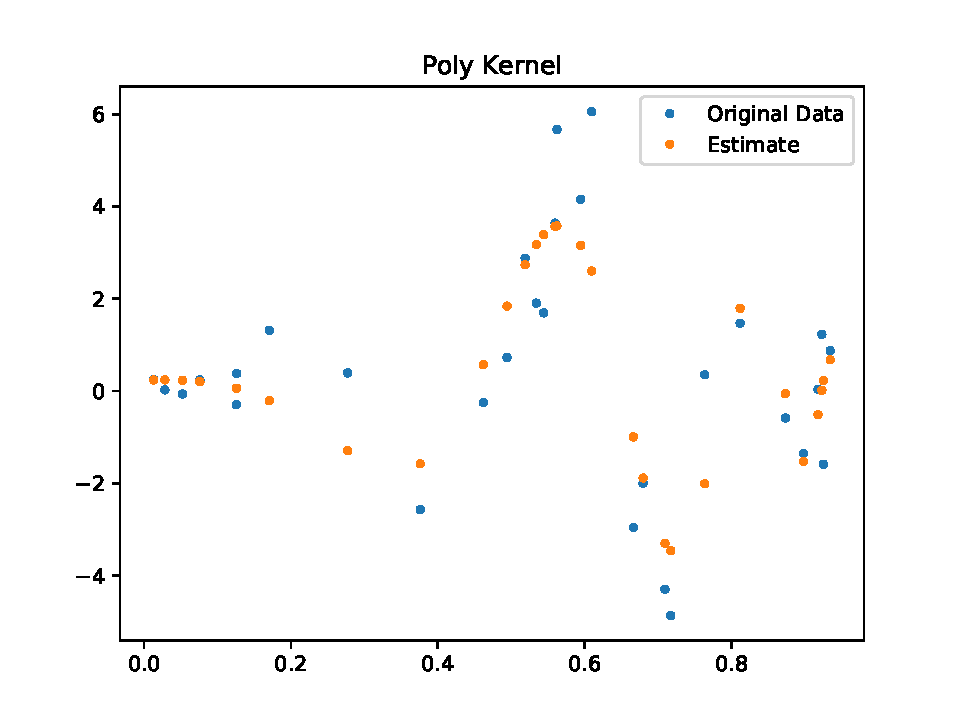
\includegraphics[width=4 in]{Figures/poly_kernel.pdf}\\
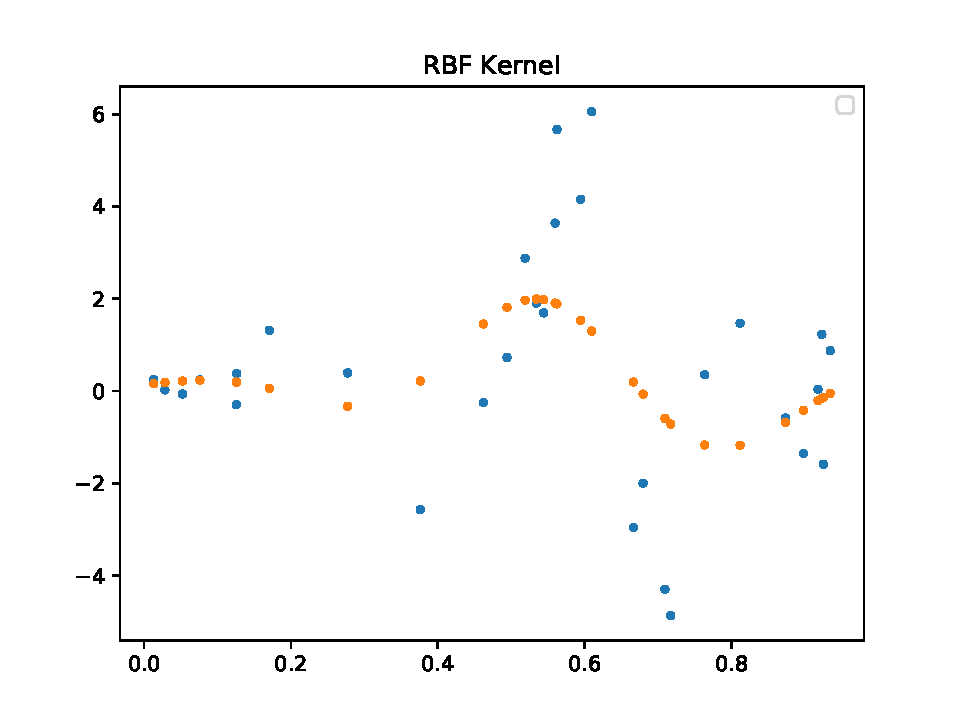
\includegraphics[width=4 in]{Figures/rbf_kernel.pdf}  


  \item Using the fixed hyperparameters you found in part a, we wish to build Bootstrap percentile confidence intervals for $\widehat{f}_{poly}(x)$ and $\widehat{f}_{rbf}(x)$ for all $x \in [0,1]$.
  Use the non-parametric bootstrap with $B=300$ datasets (i.e. randomly draw with replacement $n$ samples from $\{(x_i,y_i)\}_{i=1}^n$ and train an $\widehat{f}$, repeat this $B$ times) and find $5\%$ and $95\%$ percentiles (see Hastie, Tibshirani, Friedman Ch. 8.2 for a review). Plot the precentile curves on the plots from part b.
  \item Repeat all parts of this problem with $n=300$ (you may just use 10-fold CV instead of leave-one-out)

  \item Suppose $m$ additional samples are drawn i.i.d. the same way the first $n$ samples were drawn. Propose a statistical significance test to decide which learned function (which kernel) is the better fit (hint: if $\epsilon_i \sim \mathcal{N}(0,1)$, how is $\sum_i \epsilon_i^2$ distributed?).
\end{enumerate}
\textbf{Code:}
\begin{lstlisting}[language=Python]
import numpy as np
import matplotlib.pyplot as plt
from mpl_toolkits.mplot3d import Axes3D


def generate_data(n):

    x = np.random.uniform(0, 1, n)
    y = 4*np.sin(np.pi*x)*np.cos(6*np.pi*(x**2)) + np.random.randn(n)

    return x, y


def regress(K, y, lamb):

    try:
        a = np.linalg.solve(np.dot(K.T, K) + lamb*K, np.dot(K.T, y))

    except np.linalg.LinAlgError:
        a = np.zeros(K.shape[0])
        print('Err')

    return a


def k_poly(x, z, d):

    k = (1 + np.outer(x, z)) ** d

    return k


def cross_val_poly(x, y):

    d_n = 50
    lamb_n = 20
    errList = np.zeros((lamb_n, d_n))
    bestErr=10**100
    bestD=0
    bestLamb=0
    for d in range(1, d_n):
        for lamb in range(1, lamb_n):
            err = 0
            for i in range(len(x)):
                try:
                    a = regress(k_poly(np.delete(x, i), np.delete(x, i), d), np.delete(y, i), lamb)
                    f = np.dot(a, k_poly(np.delete(x, i), x[i], d))
                    err += (f-y[i])**2

                except np.linalg.linalg.LinAlgError:
                    err = np.inf
            print(err)
            errList[lamb, d] = err
            if err<bestErr:
                bestD = d
                bestLamb = lamb
                bestErr = err

    plt.figure()
    X, Y = np.meshgrid(range(0, d_n), range(0, lamb_n))
    ax = plt.axes(projection='3d')
    ax.plot_surface(X, Y, np.log10(errList))
    plt.xlabel('d')
    plt.ylabel('lambda')
    plt.draw()
    return bestD, bestLamb


def boot_poly(x, y, d, lamb, n):

    f = np.zeros((n, x.size))
    for inter in range(n):

        i_cut = np.random.choice(x.size, x.size)
        x_cut = x[i_cut]
        y_cut = y[i_cut]
        try:
            a = regress(k_poly(x_cut, x_cut, d), y_cut, lamb)
            f[inter] = np.dot(a, k_poly(x_cut, x_cut, d))

        except np.linalg.LinAlgError:
            print('Err')

    return f

def k_rbf(x, z, gam):

    k=np.zeros((x.size,z.size))
    for i in range(x.size):
        for j in range(z.size):
            if(z.size>1):
                k[i,j] = np.exp(-gam*np.dot(x[i]-z[j], x[i]-z[j]))
            else:
                k[i]=np.exp(-gam*np.sum(np.dot(x[i]-z, x[i]-z)))
    return k


def cross_val_rbf(x, y):

    gam_n = 20
    lamb_n = 20
    errList = np.zeros((lamb_n, gam_n))
    bestErr=10**100
    bestGam=0
    bestLamb=0

    for gam in range(1, gam_n):
        for lamb in range(1, lamb_n):
            err = 0
            for i in range(len(x)):
                try:
                    a = regress(k_rbf(np.delete(x, i), np.delete(x, i), gam), np.delete(y, i), lamb)
                    f = np.dot(a, k_rbf(np.delete(x, i), x[i], gam))
                    err += (f-y[i])**2

                except np.linalg.linalg.LinAlgError:
                    err = np.inf
            print(err)
            errList[lamb, gam]=err
            if err<bestErr:
                bestGam = gam
                bestLamb = lamb
                bestErr = err

    plt.figure()
    X, Y = np.meshgrid(range(0, gam_n), range(0, lamb_n))
    ax = plt.axes(projection='3d')
    ax.plot_surface(X, Y, np.log10(errList))
    plt.draw()
    return bestGam, bestLamb

x, y = generate_data(30)

d, lamb =cross_val_poly(x, y)
a = regress(k_poly(x, x, d), y, lamb)
f = np.dot(a, k_poly(x, x, d))

print('d: ' + str(d))
print('Lambda: ' + str(lamb))
# boot_f = boot_poly(x, y, d, lamb, 10)


plt.figure()
plt.plot(x, y, '.')
plt.plot(x, f, '.')
plt.legend(('Original Data', 'Estimate'))
plt.title('Poly Kernel')
plt.savefig('Figures/poly_kernel.pdf')
plt.draw()

gam, lamb =cross_val_rbf(x, y)
a = regress(k_rbf(x, x, gam), y, lamb)
f = np.dot(a, k_rbf(x, x, gam))


print('Gamma: ' + str(gam))
print('Lambda: ' + str(lamb))

plt.figure()
plt.plot(x, y, '.')
plt.plot(x, f, '.')
plt.legend('Original Data', 'Estimate')
plt.title('RBF Kernel')
plt.savefig('Figures/rbf_kernel.pdf')
plt.draw()

x, y = generate_data(300)

d, lamb =cross_val_poly(x, y)
a = regress(k_poly(x, x, d), y, lamb)
f = np.dot(a, k_poly(x, x, d))

print('d: ' + str(d))
print('Lambda: ' + str(lamb))
# boot_f = boot_poly(x, y, d, lamb, 10)

plt.show()




\end{lstlisting}

\section{$k$-means clustering}

4. \grade{5} Given a dataset $x_1,..., x_n \in \R^{d}$ and an integer $1 \leq k \leq n$, recall the following $k$-means objective function
\begin{align}
    \min_{\pi_1, ..., \pi_k} \sum_{i=1}^{k} \sum_{j \in \pi_i} \norm{ x_j - \mu_{i} }^2_2 \ , \quad \mu_i = \frac{1}{|\pi_i|} \sum_{j \in \pi_i} x_j \ . \label{eq:kmeans_obj}
\end{align}
Above, $\{\pi_i\}_{i=1}^{k}$ is a partition of $\{1, 2, ..., n\}$. The objective \eqref{eq:kmeans_obj} is NP-hard\footnote{
To be more precise, it is both NP-hard in $d$ when $k=2$ and $k$ when $d=2$.
See the references on the wikipedia page for $k$-means for more details.
} to find a global minimizer of. Nevertheless the commonly used heuristic which we discussed in lecture, known as Lloyd's algorithm, typically works well in practice.
Implement Lloyd's algorithm for solving the $k$-means objective \eqref{eq:kmeans_obj}.
Do not use any off the shelf implementations, such as those found in \texttt{scikit-learn}.
\begin{enumerate}
    \item Run the algorithm on MNIST with $k=5,10,20$, plotting the objective function \eqref{eq:kmeans_obj} as a function of iteration. Visualize (and include in your report) the cluster centers as a $28\times 28$ image.
    
    \textbf{Answer:}\\
    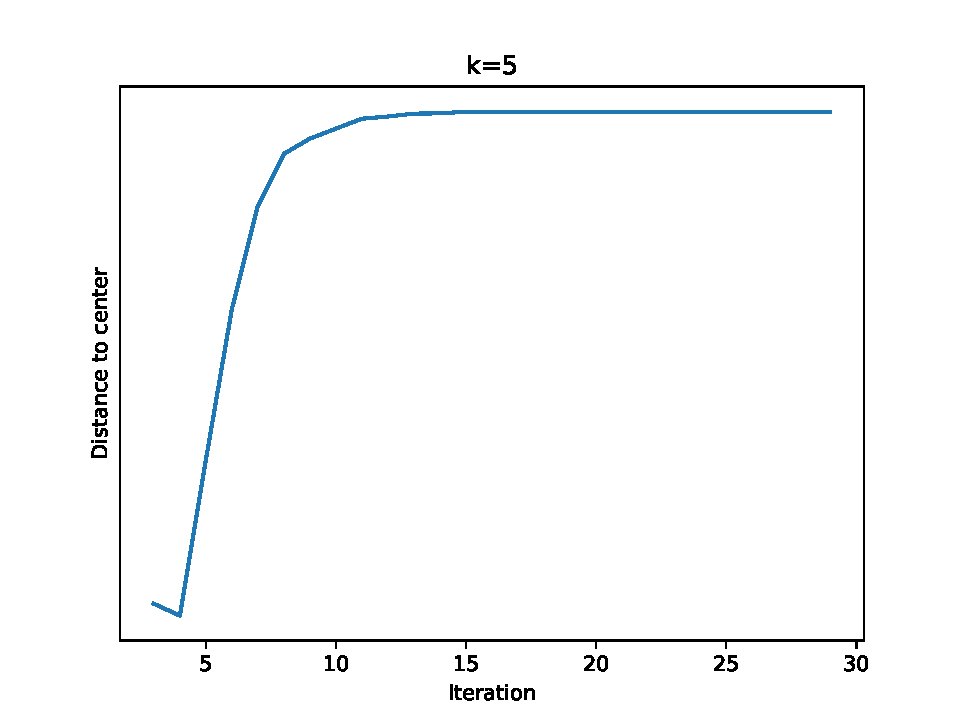
\includegraphics[width=4 in]{Figures/error5.pdf}\\
    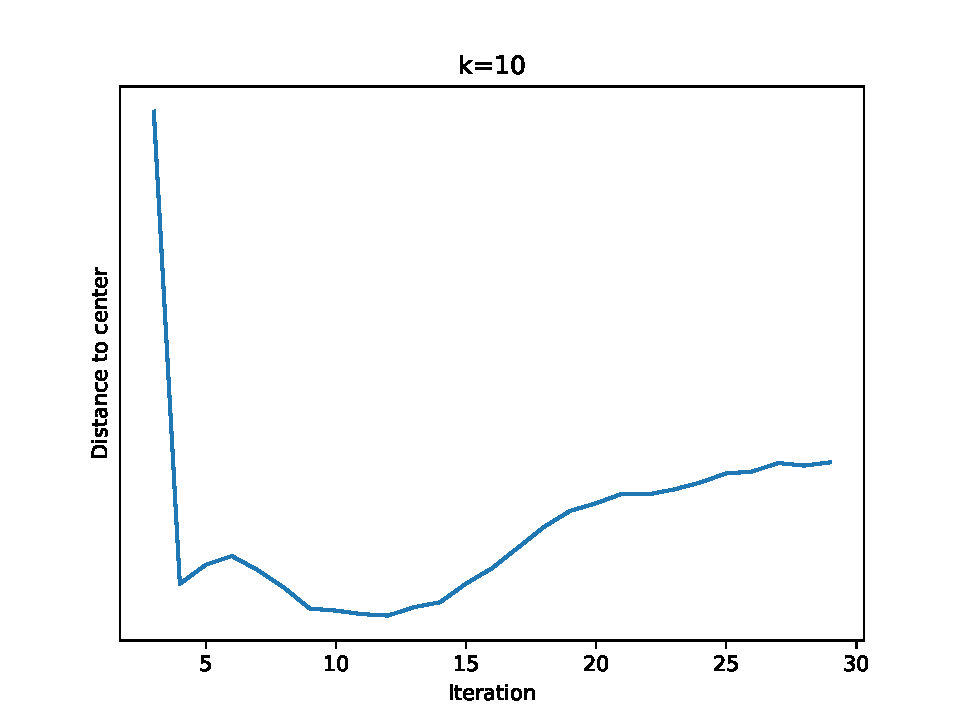
\includegraphics[width=4 in]{Figures/error10.pdf}\\
    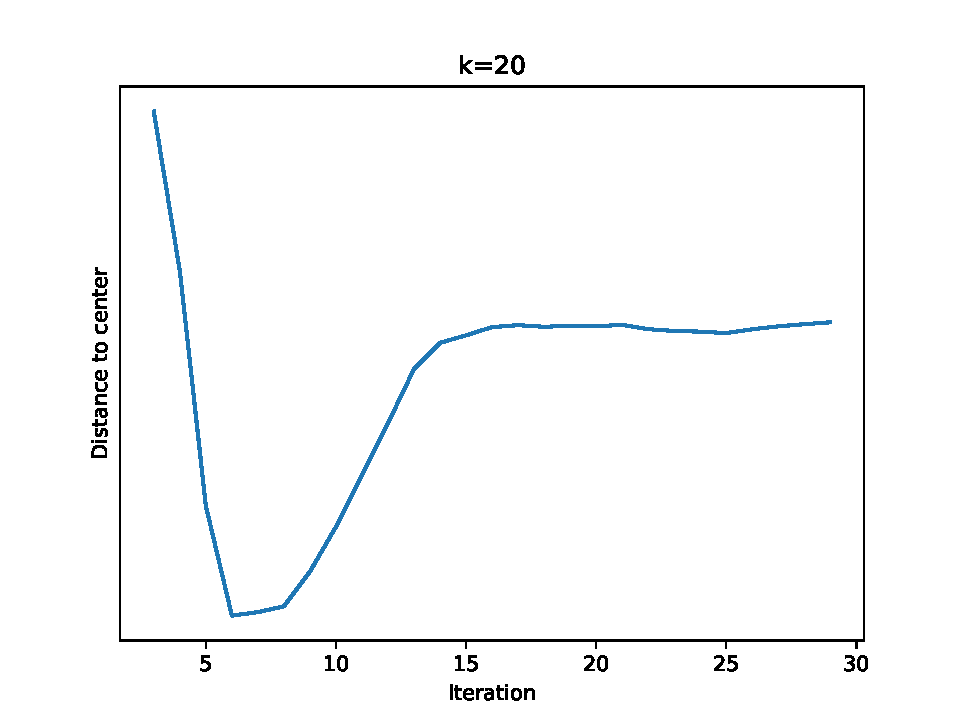
\includegraphics[width=4 in]{Figures/error20.pdf}\\
    
    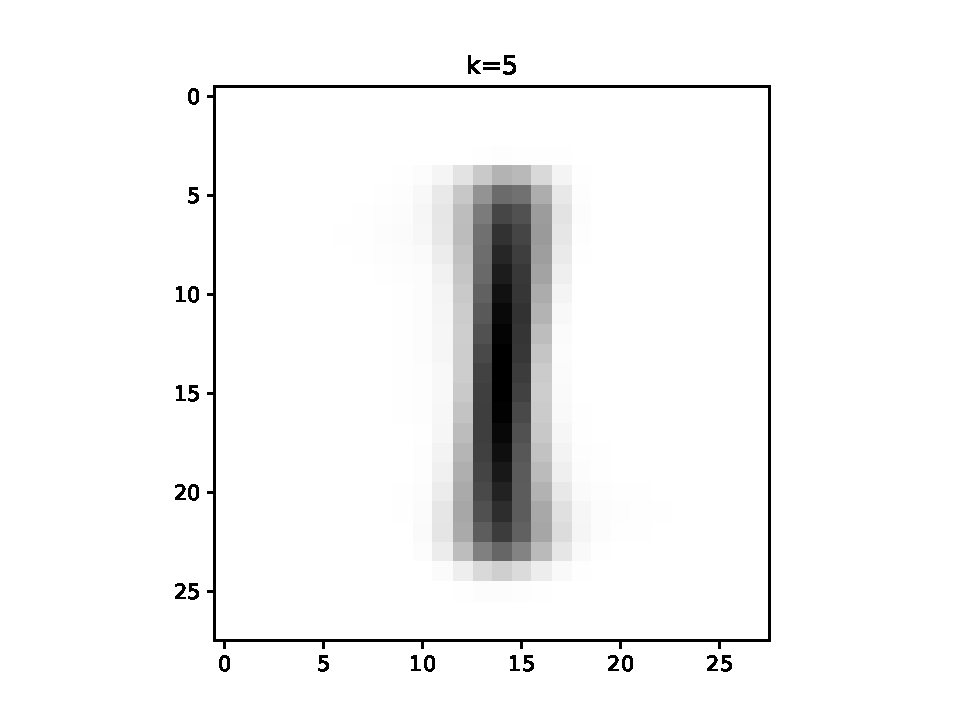
\includegraphics[width=2 in]{Figures/means5_0.pdf}    
    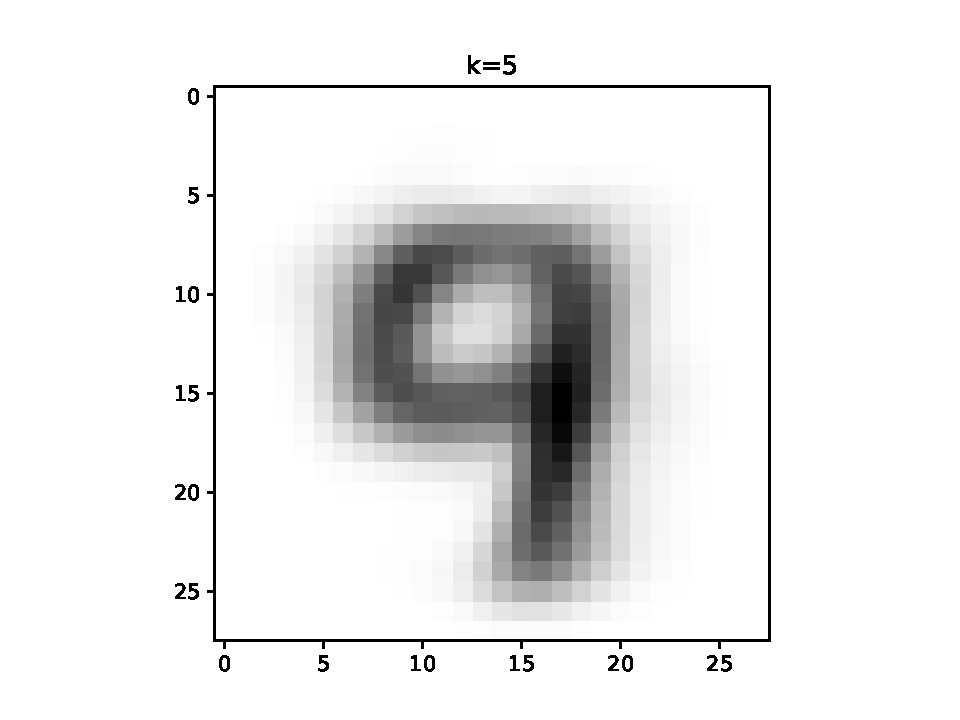
\includegraphics[width=2 in]{Figures/means5_1.pdf}    
    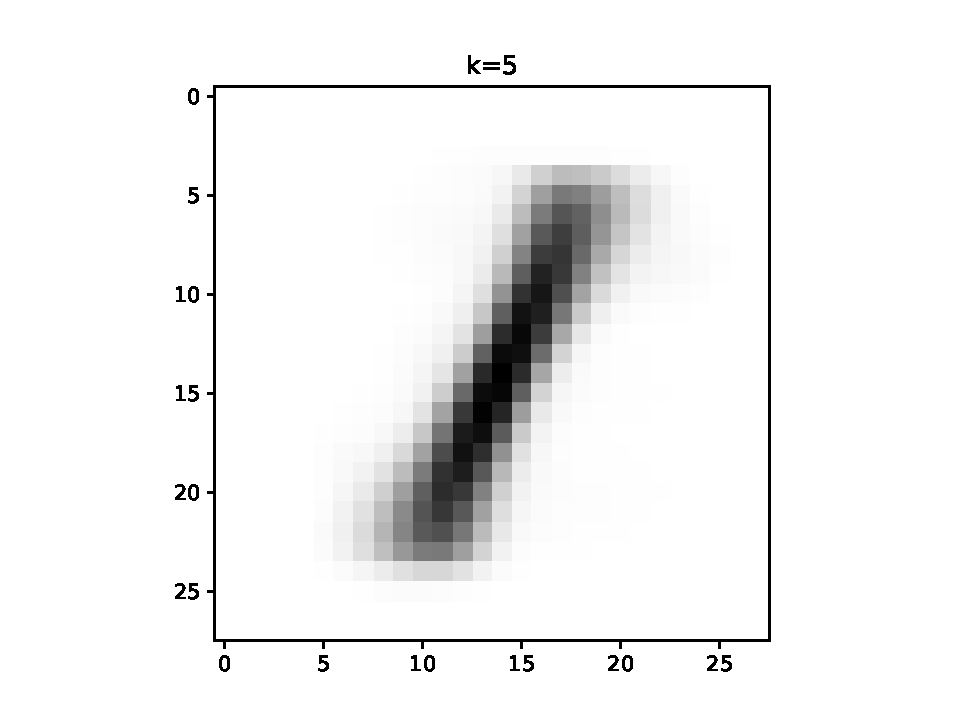
\includegraphics[width=2 in]{Figures/means5_2.pdf}\\
     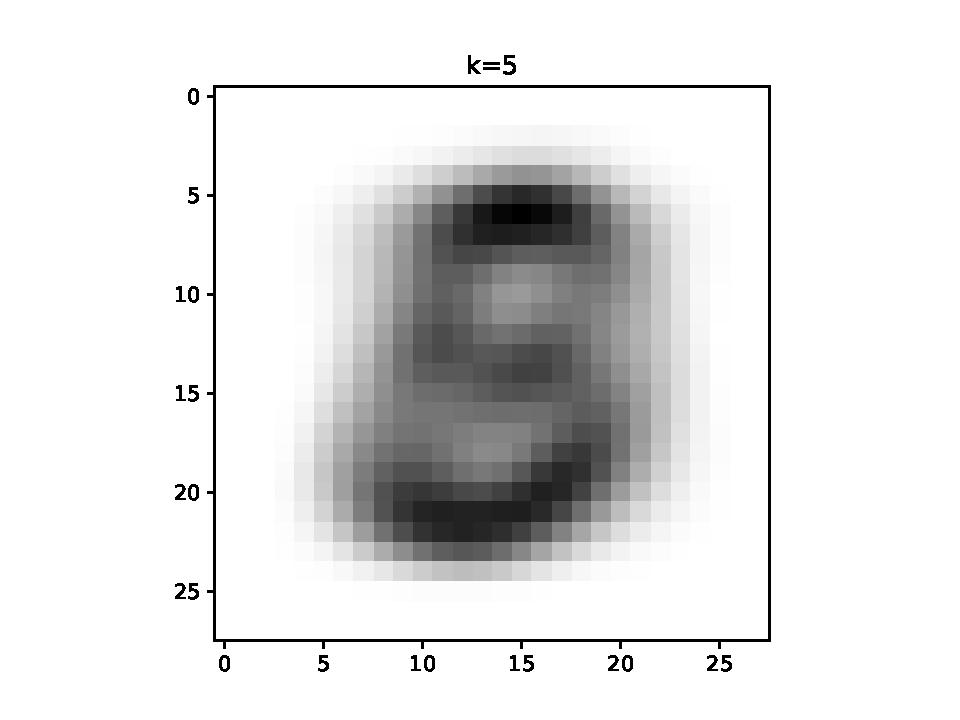
\includegraphics[width=2 in]{Figures/means5_3.pdf}    
    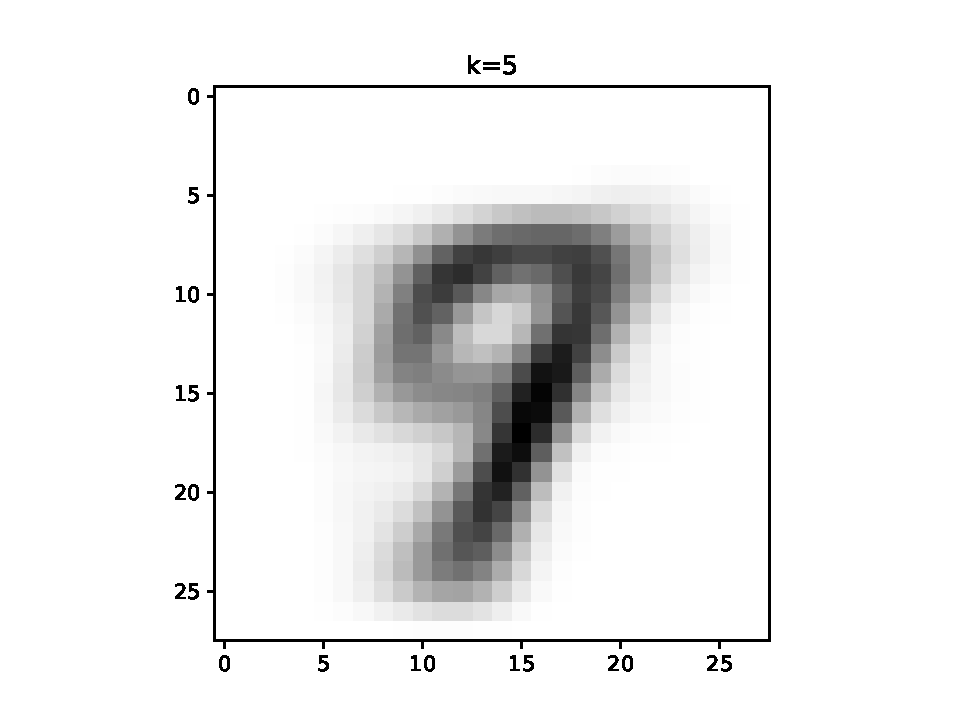
\includegraphics[width=2 in]{Figures/means5_4.pdf} \\
    
     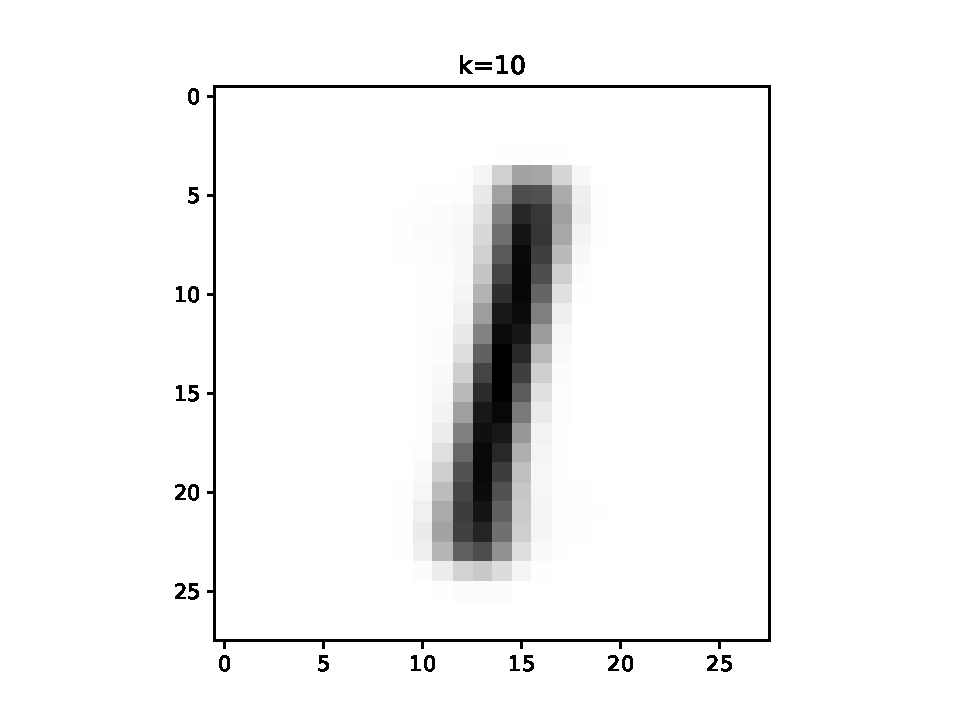
\includegraphics[width=2 in]{Figures/means10_0.pdf}    
    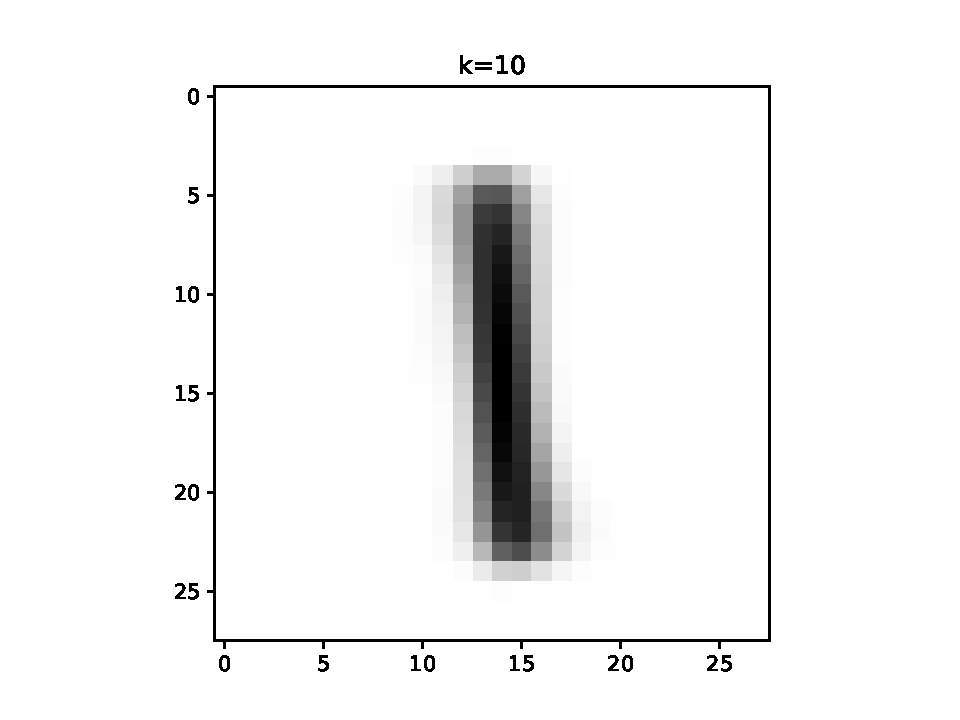
\includegraphics[width=2 in]{Figures/means10_1.pdf}    
    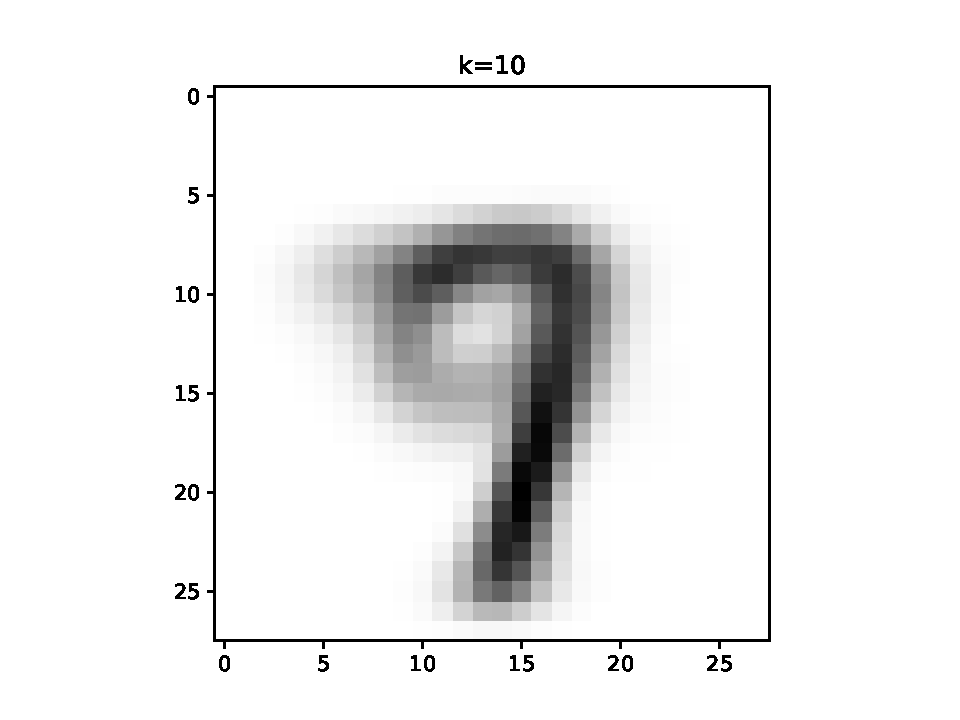
\includegraphics[width=2 in]{Figures/means10_2.pdf}\\
     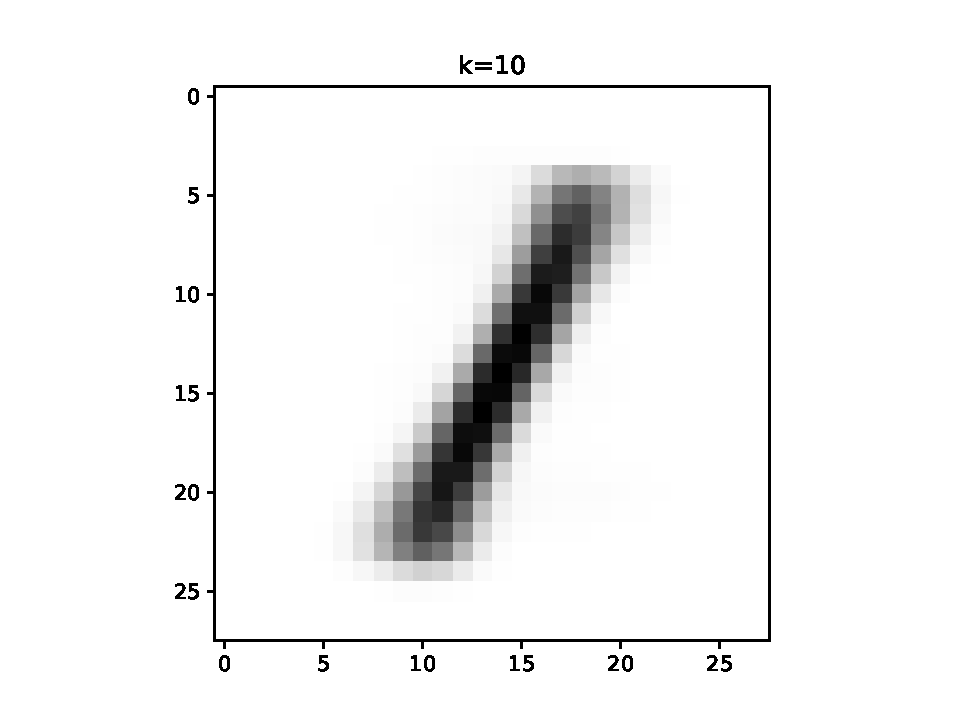
\includegraphics[width=2 in]{Figures/means10_3.pdf}    
    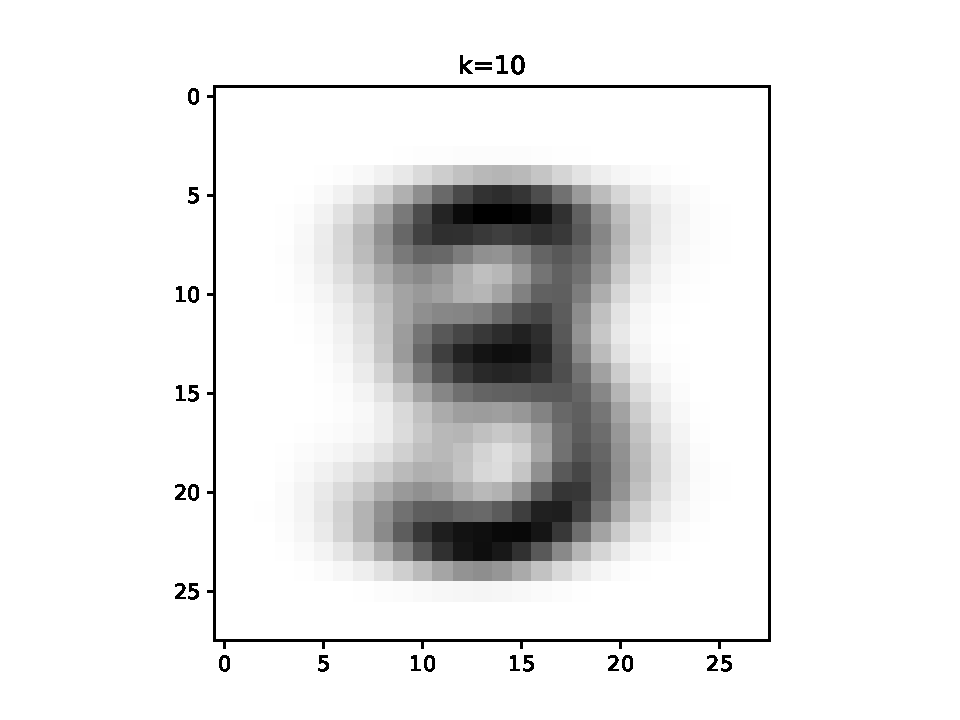
\includegraphics[width=2 in]{Figures/means10_4.pdf} 
     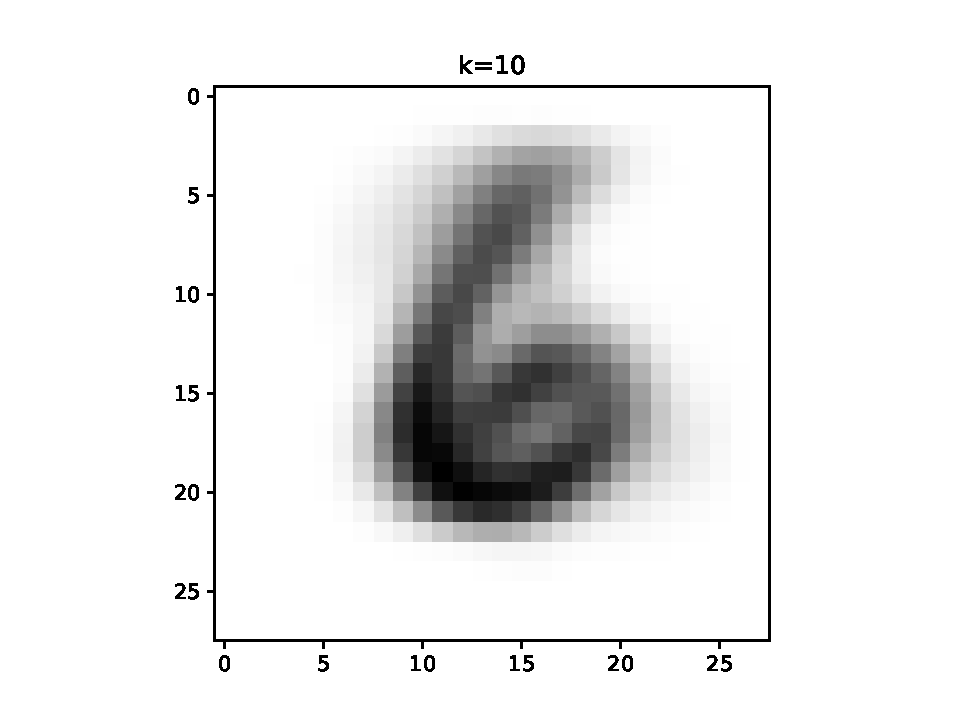
\includegraphics[width=2 in]{Figures/means10_5.pdf}   \\
    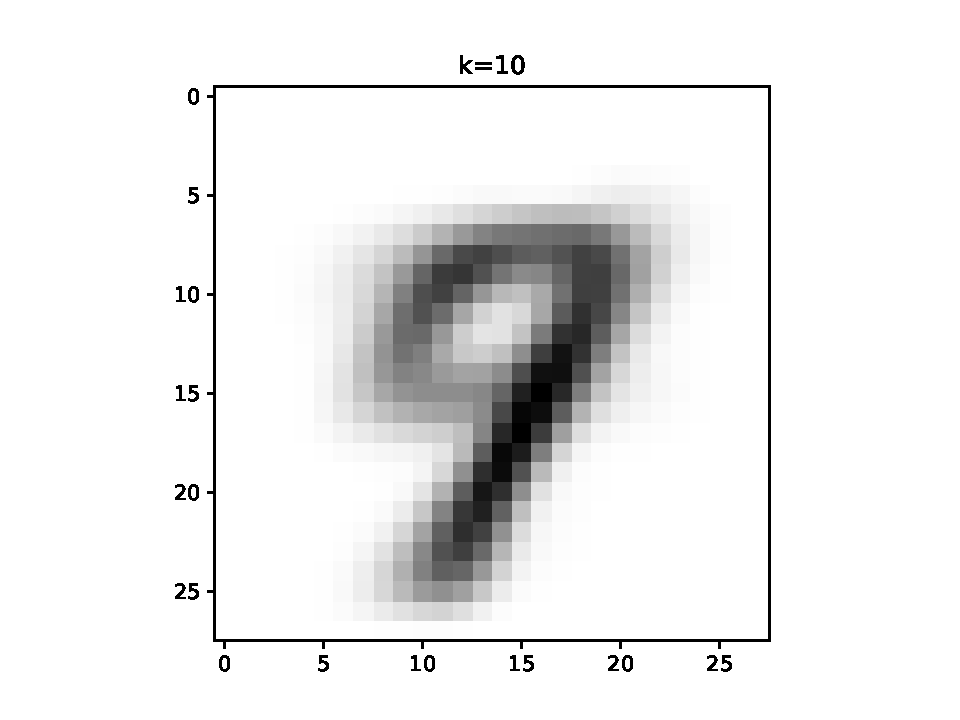
\includegraphics[width=2 in]{Figures/means10_6.pdf}    
    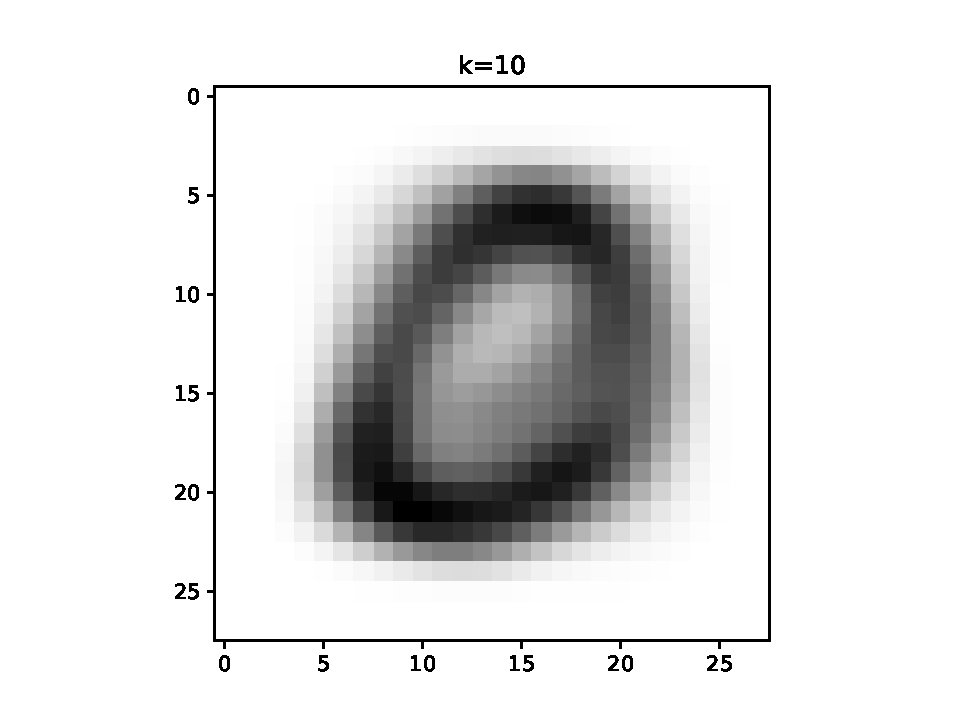
\includegraphics[width=2 in]{Figures/means10_7.pdf}
     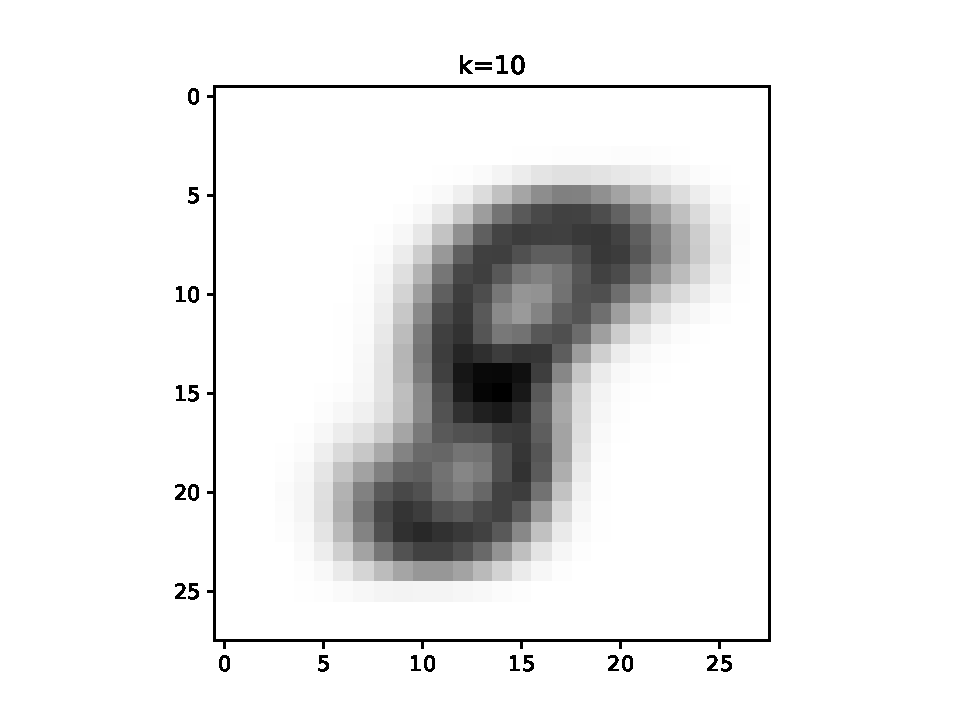
\includegraphics[width=2 in]{Figures/means10_8.pdf}    \\
    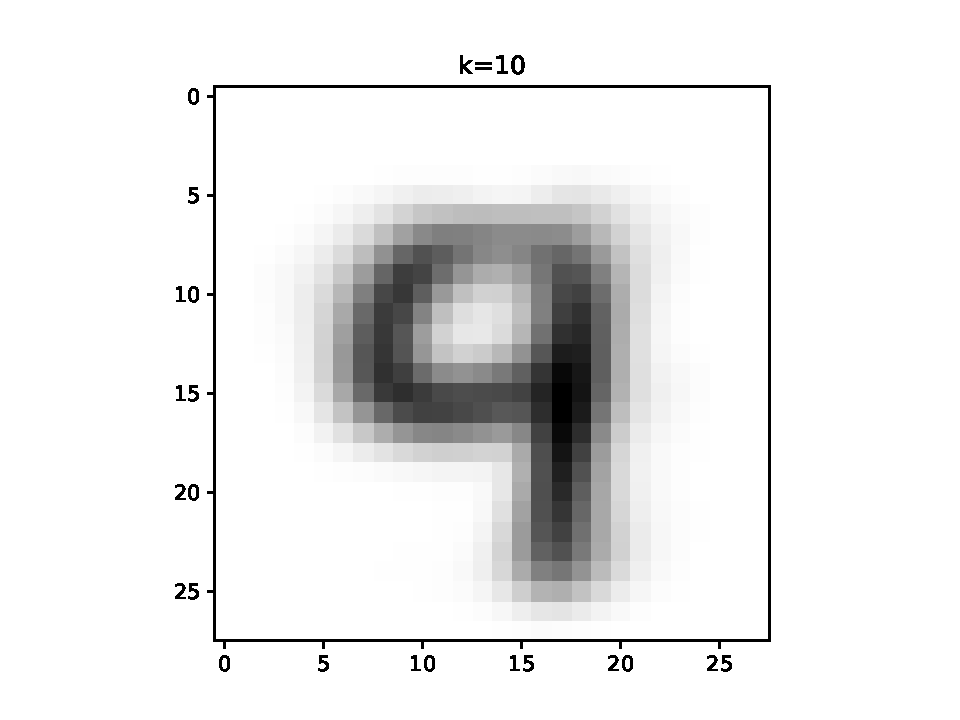
\includegraphics[width=2 in]{Figures/means10_9.pdf} \\
    
     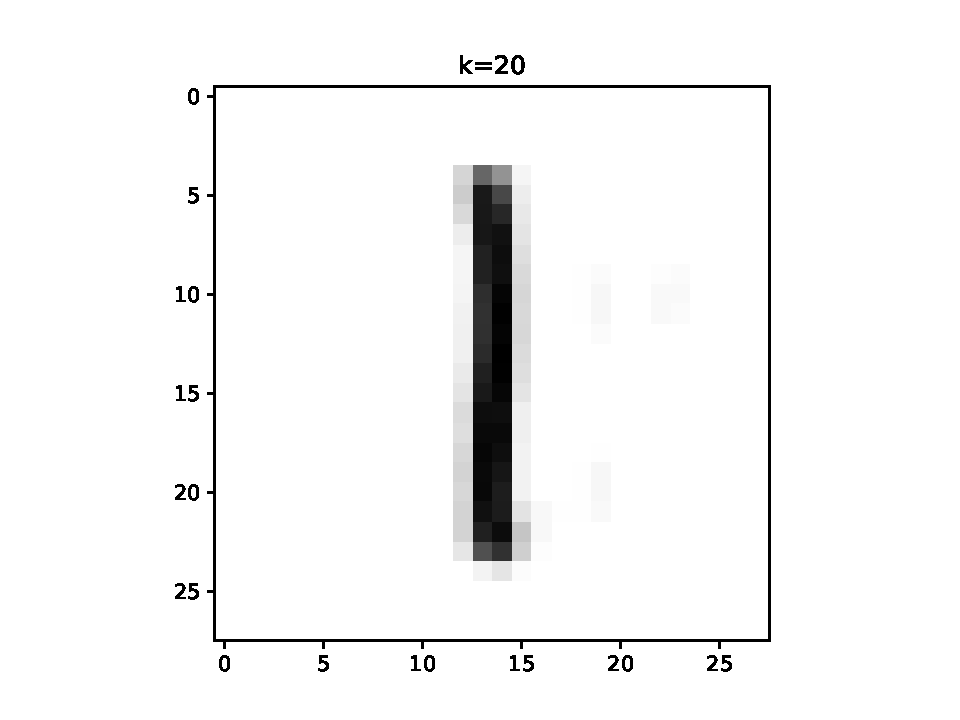
\includegraphics[width=2 in]{Figures/means20_0.pdf}    
    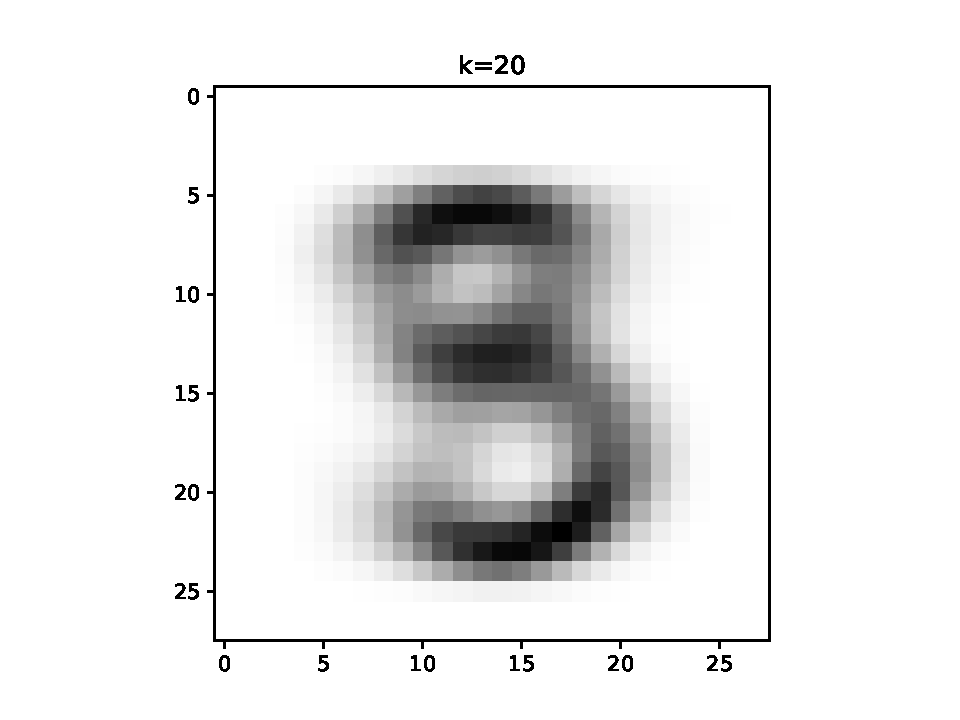
\includegraphics[width=2 in]{Figures/means20_1.pdf}    
    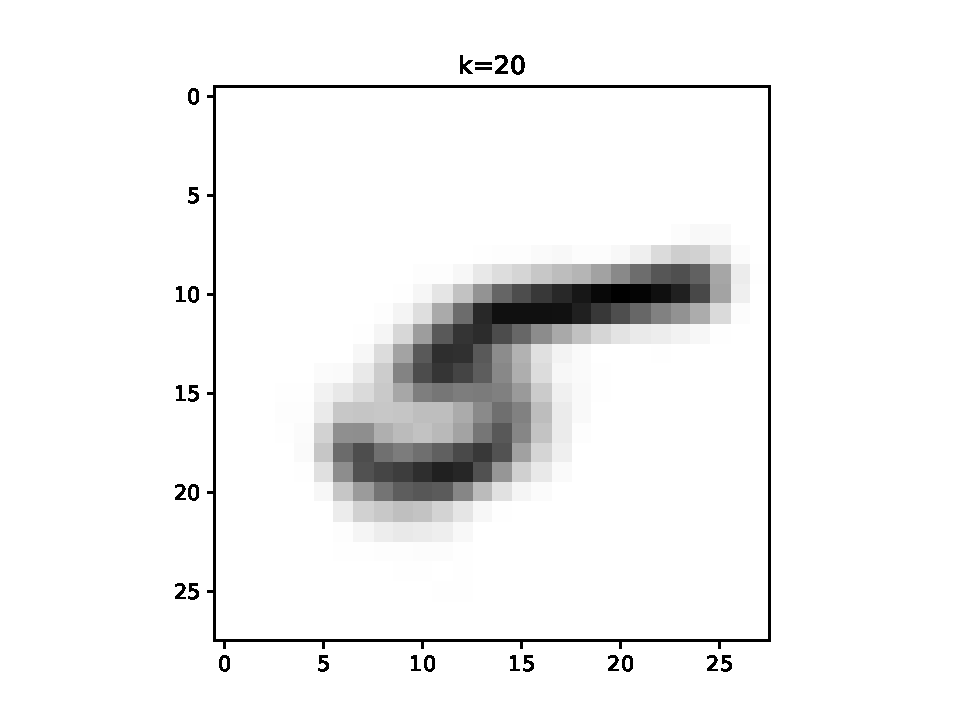
\includegraphics[width=2 in]{Figures/means20_2.pdf}\\
     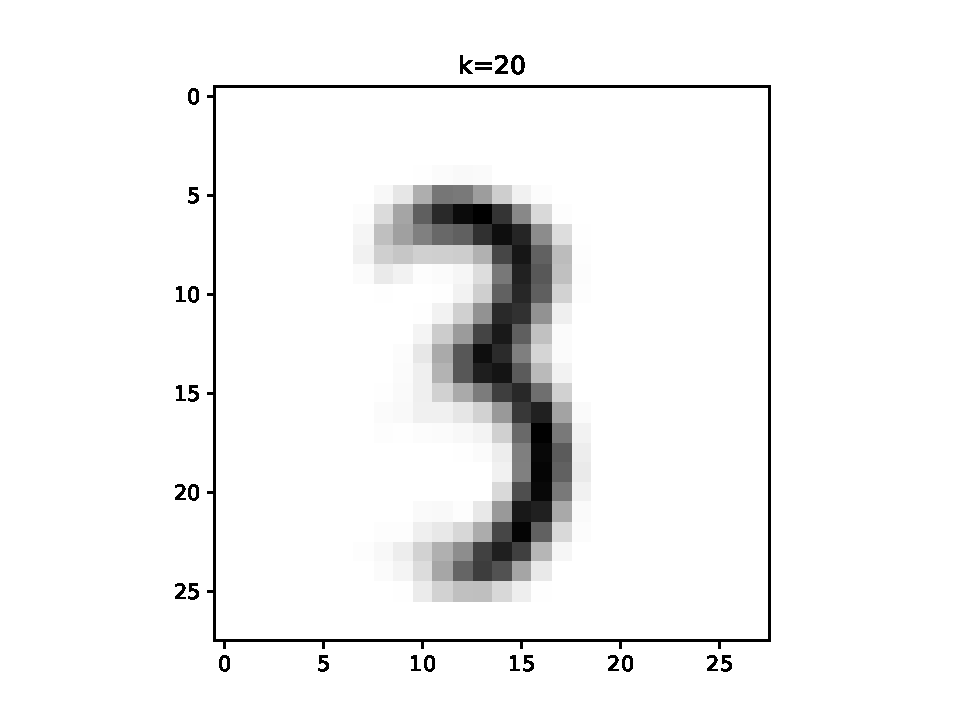
\includegraphics[width=2 in]{Figures/means20_3.pdf}    
    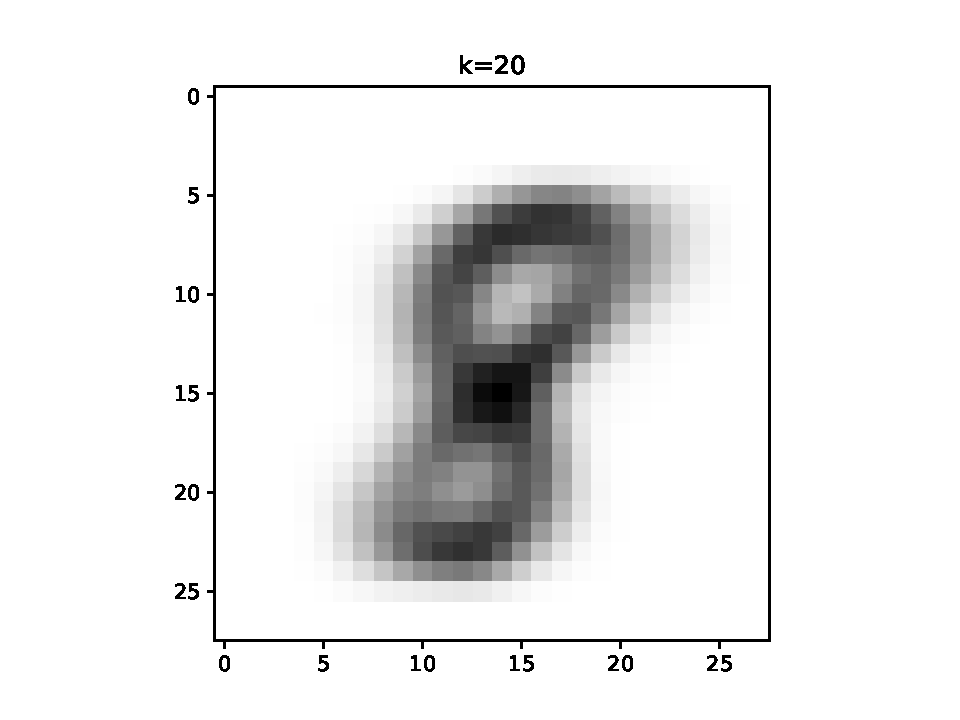
\includegraphics[width=2 in]{Figures/means20_4.pdf} 
     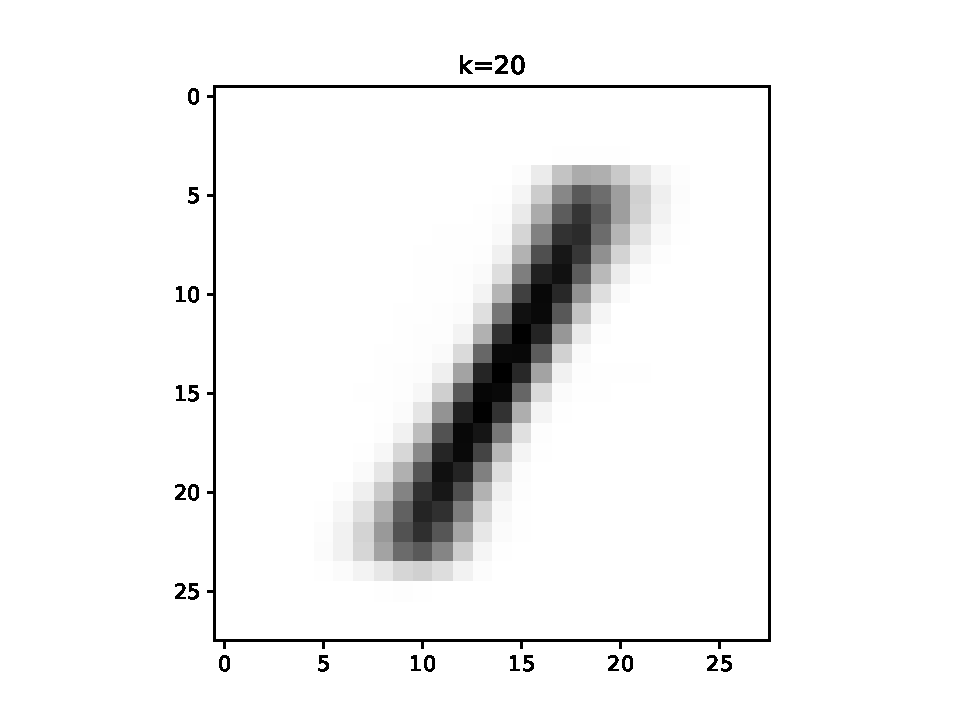
\includegraphics[width=2 in]{Figures/means20_5.pdf}   \\
    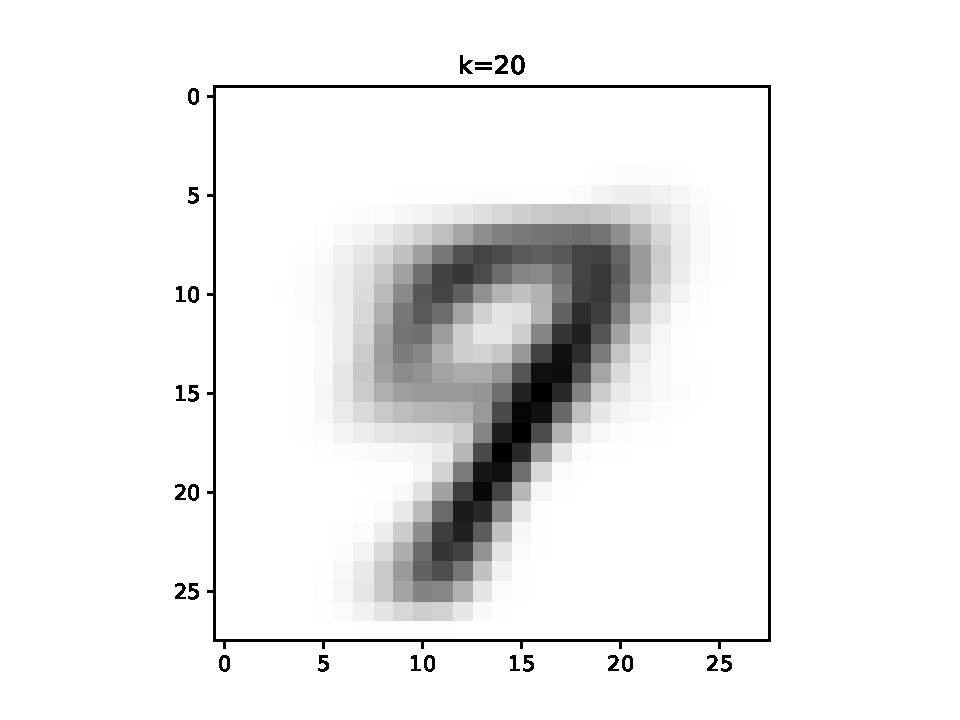
\includegraphics[width=2 in]{Figures/means20_6.pdf}    
    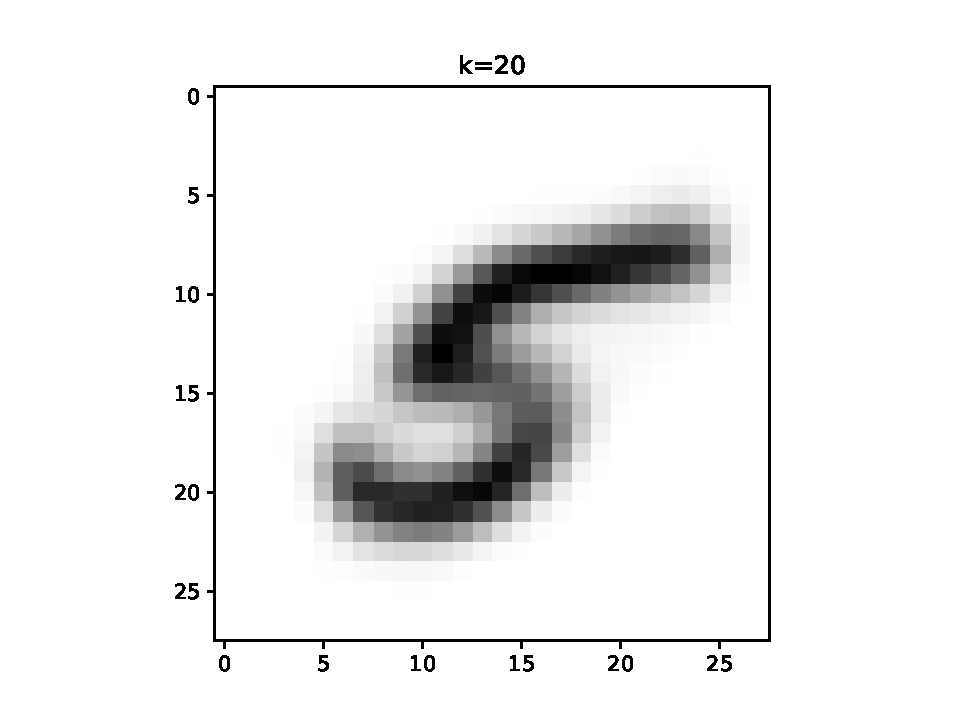
\includegraphics[width=2 in]{Figures/means20_7.pdf}
     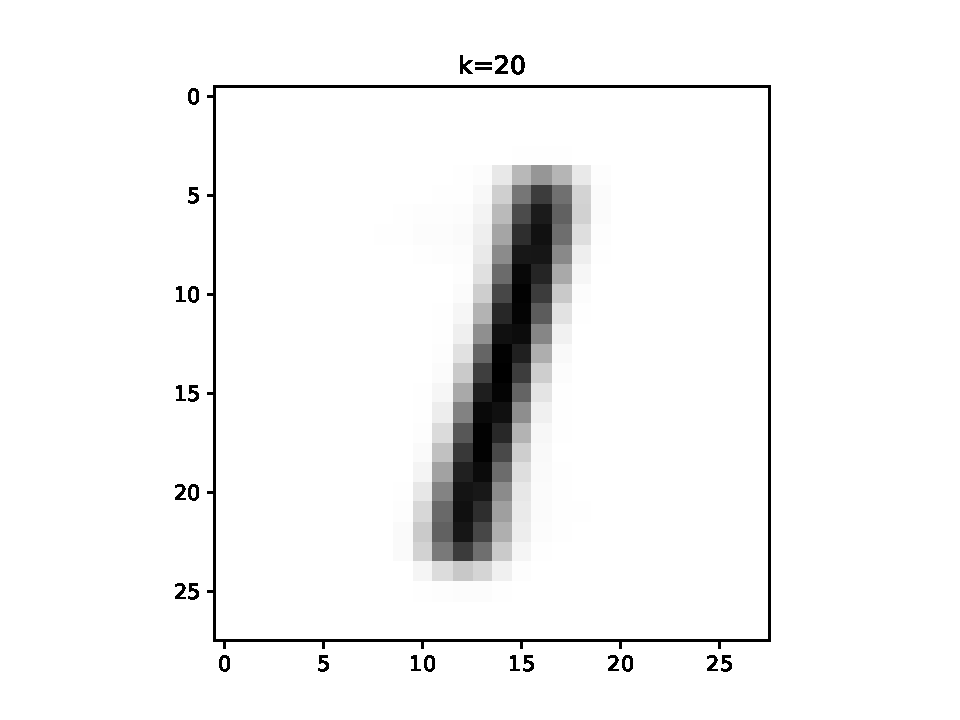
\includegraphics[width=2 in]{Figures/means20_8.pdf}    \\
    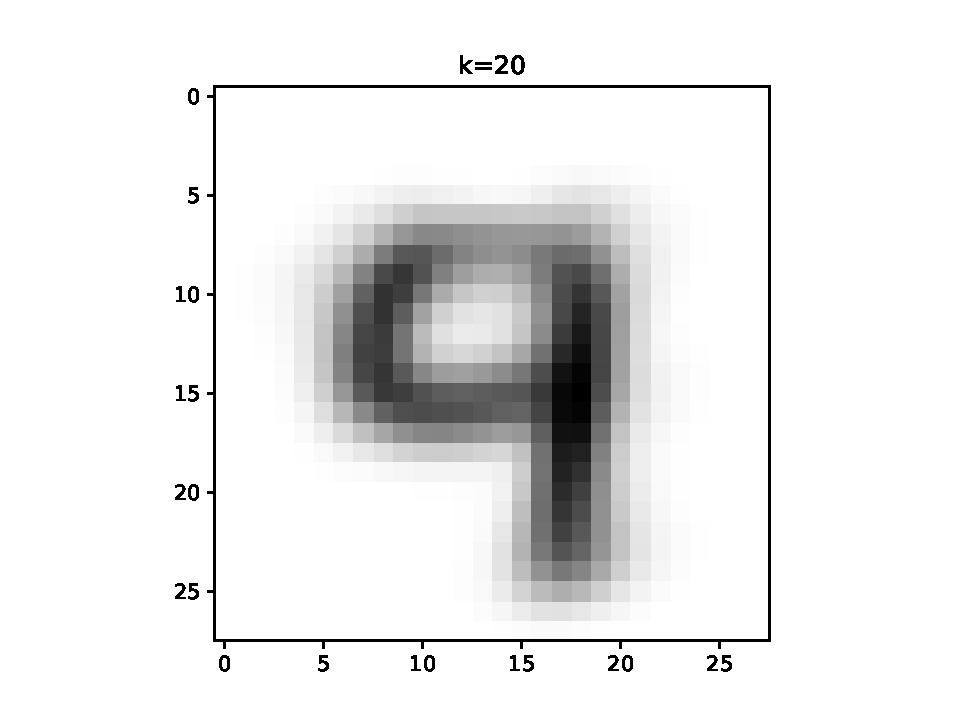
\includegraphics[width=2 in]{Figures/means20_9.pdf} 
       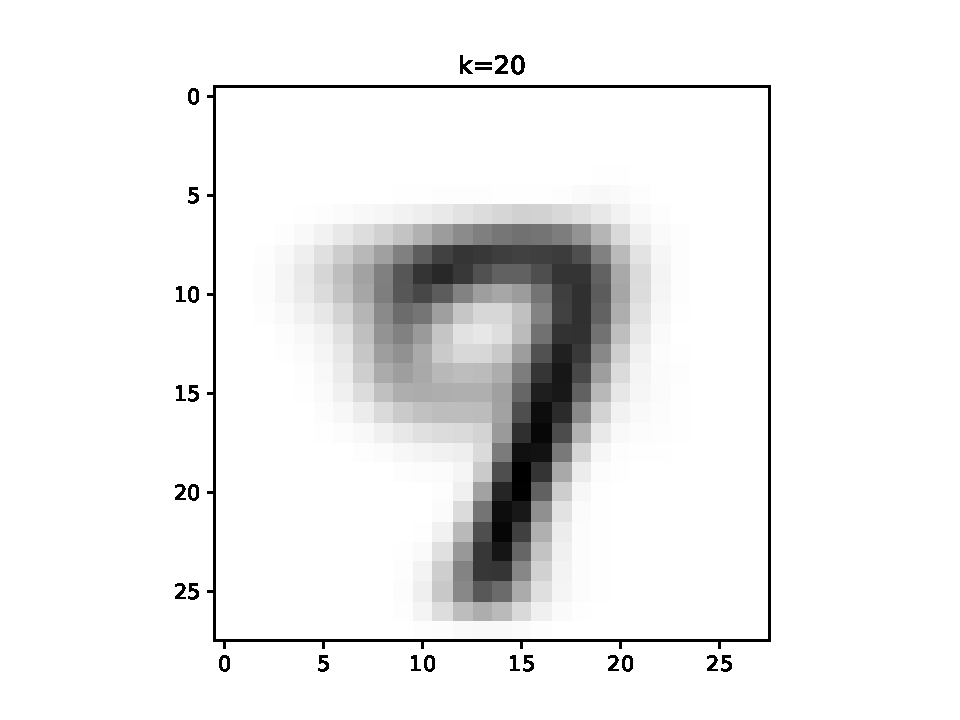
\includegraphics[width=2 in]{Figures/means20_10.pdf}    
    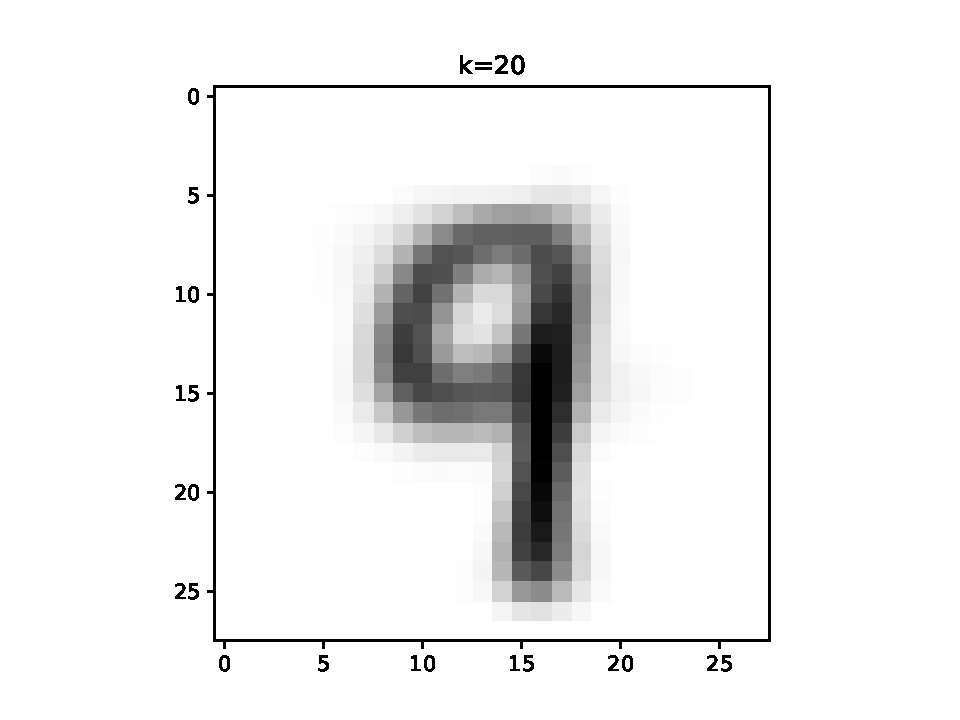
\includegraphics[width=2 in]{Figures/means20_11.pdf}    \\
    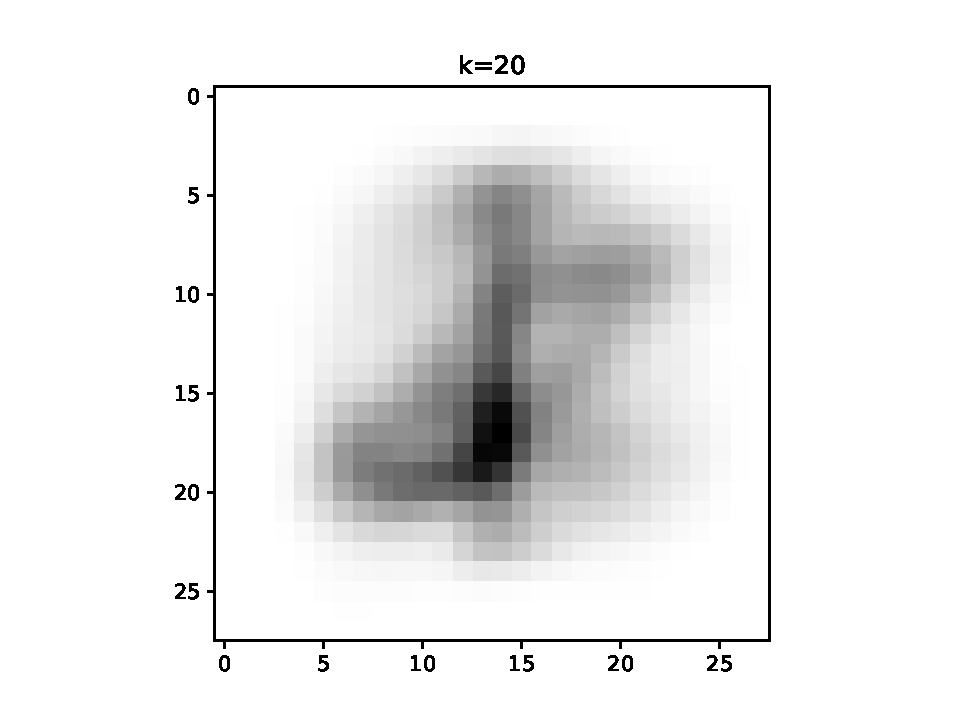
\includegraphics[width=2 in]{Figures/means20_12.pdf}
     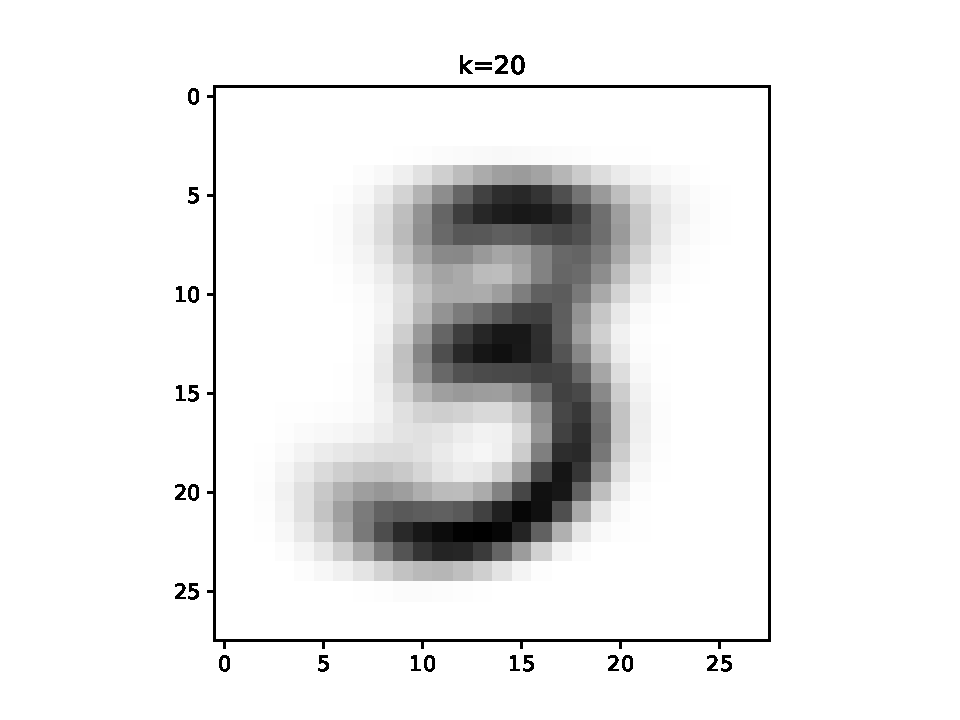
\includegraphics[width=2 in]{Figures/means20_13.pdf}    
    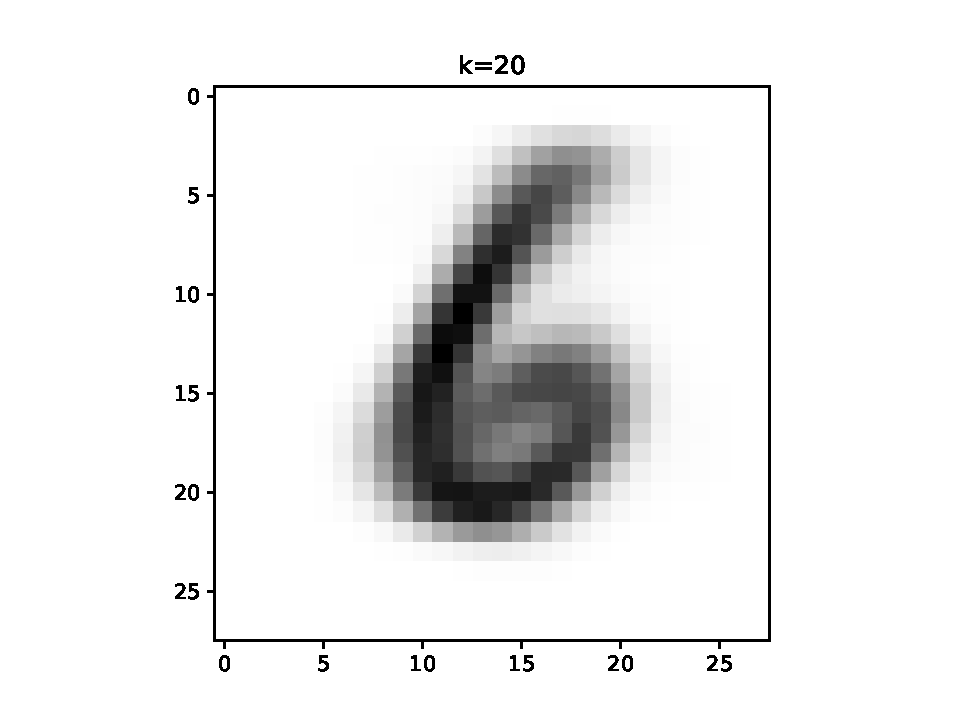
\includegraphics[width=2 in]{Figures/means20_14.pdf} \\
     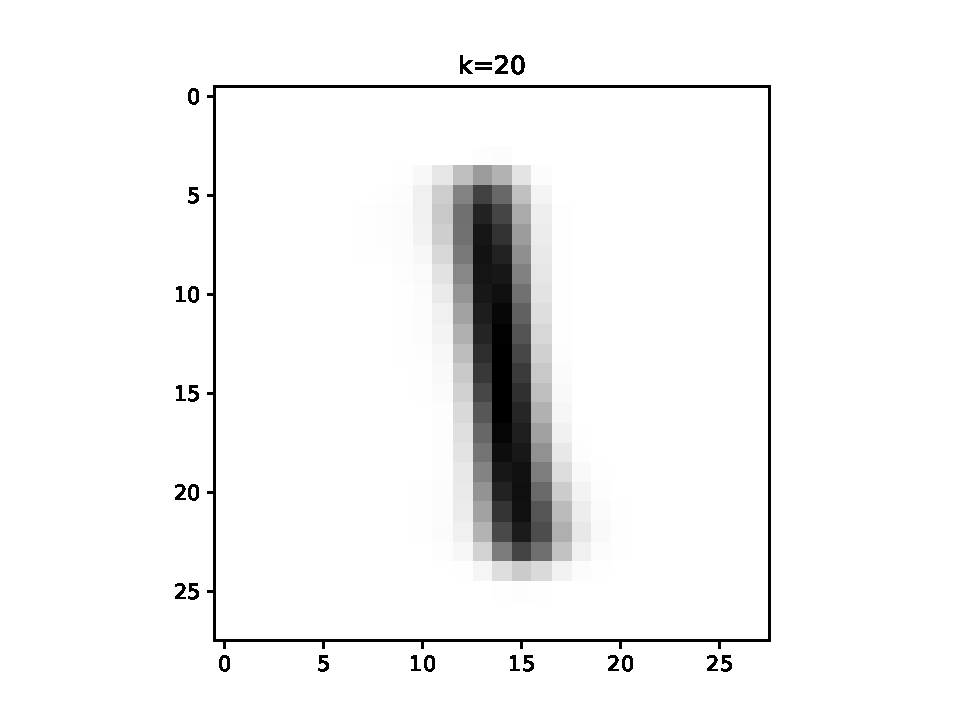
\includegraphics[width=2 in]{Figures/means20_15.pdf}   
    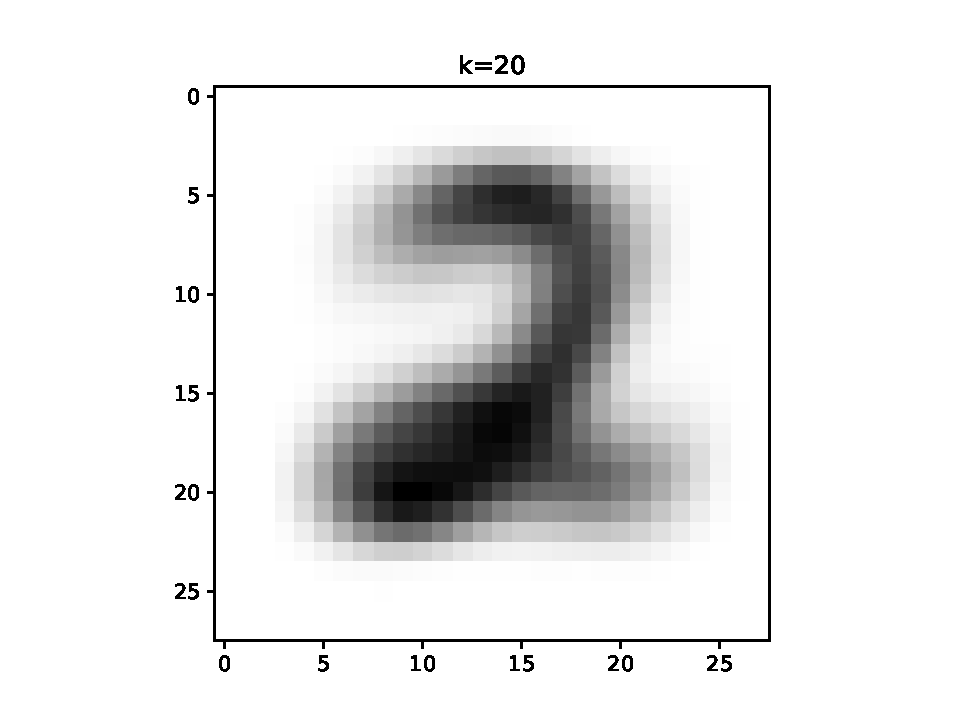
\includegraphics[width=2 in]{Figures/means20_16.pdf}    
    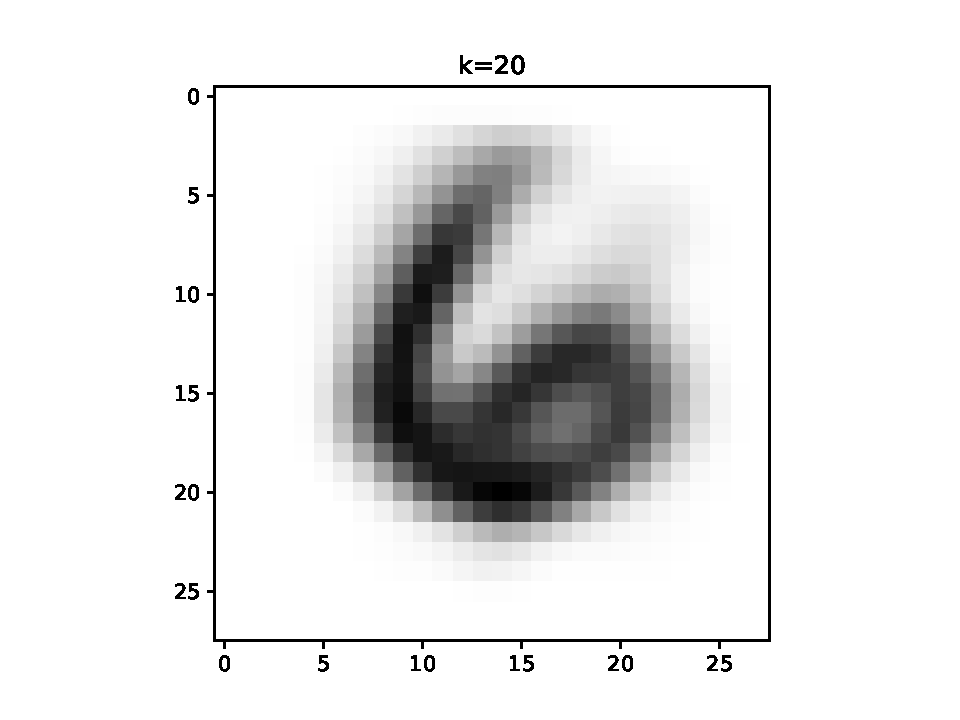
\includegraphics[width=2 in]{Figures/means20_17.pdf}\\
     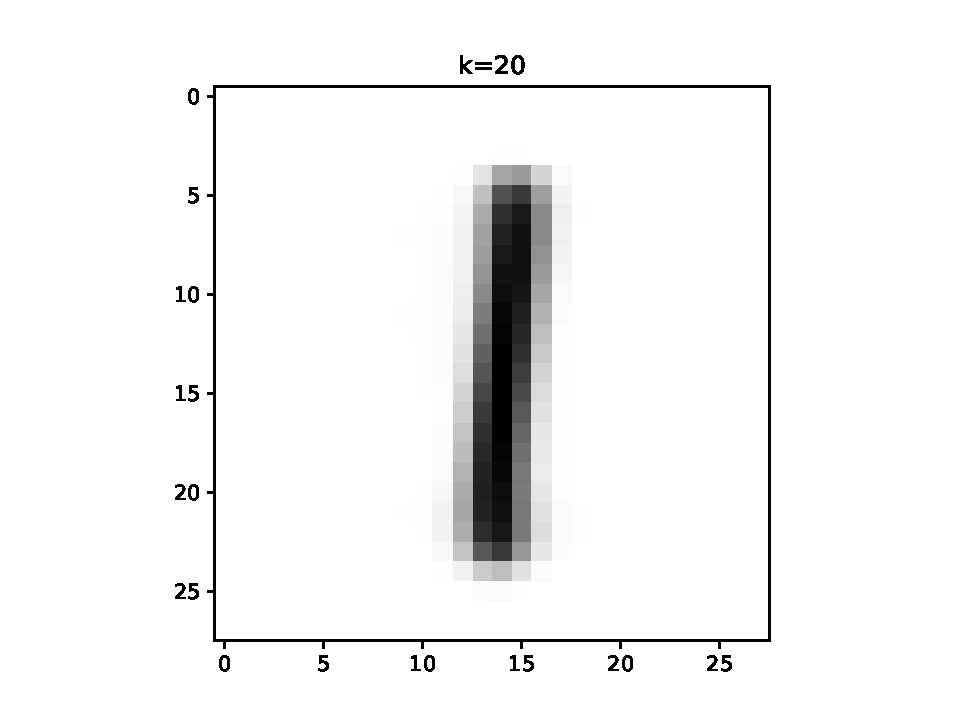
\includegraphics[width=2 in]{Figures/means20_18.pdf}  
    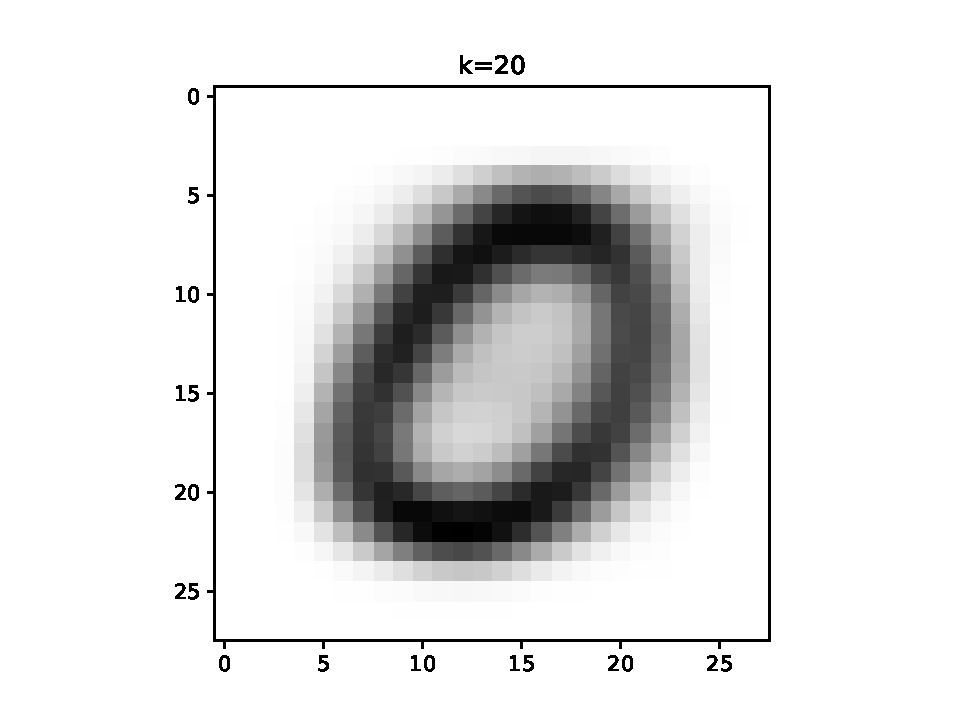
\includegraphics[width=2 in]{Figures/means20_19.pdf} \\
    
    \item Implement the \texttt{kmeans++} initialization scheme\footnote{See \url{http://ilpubs.stanford.edu:8090/778/1/2006-13.pdf}.} for your
        $k$-means implementation and repeat part a.  Note that this initialization scheme is widely used in practice, and as a rule should be used. Plot the objective function as a function of iteration. Are the identified centers visually better than part a? 
        
\textbf{Answer:}\\
The kmeans++ and kmeans centers almost the same which is odd. I would expect that an algorithm that attempts to place the centers at higher density places from the start would be better than randomly sampling.

    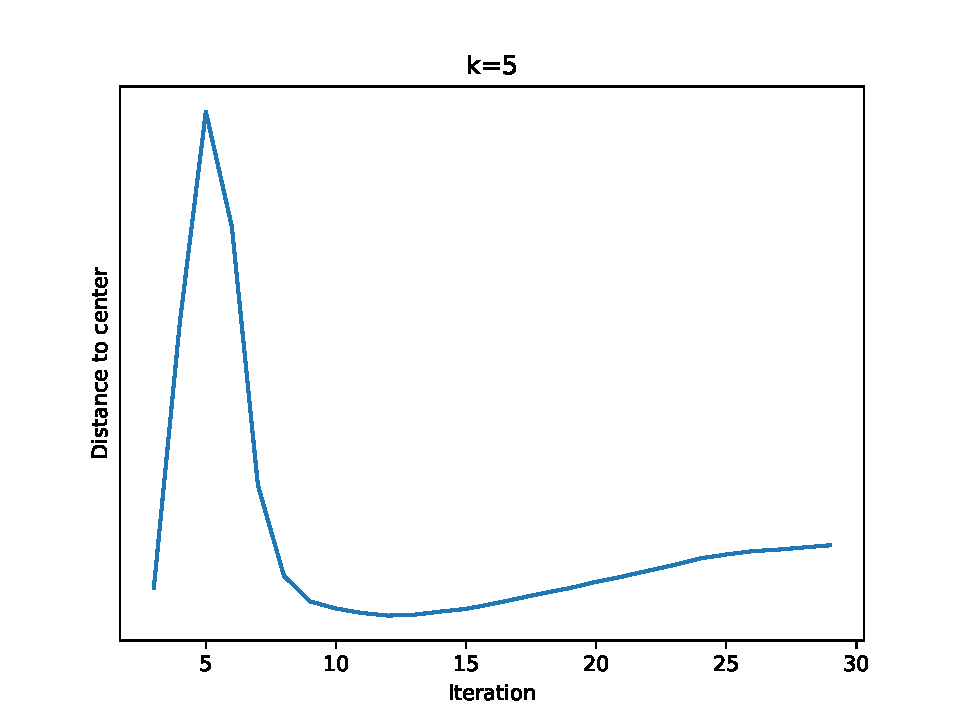
\includegraphics[width=4 in]{Figures/error++5.pdf}\\
    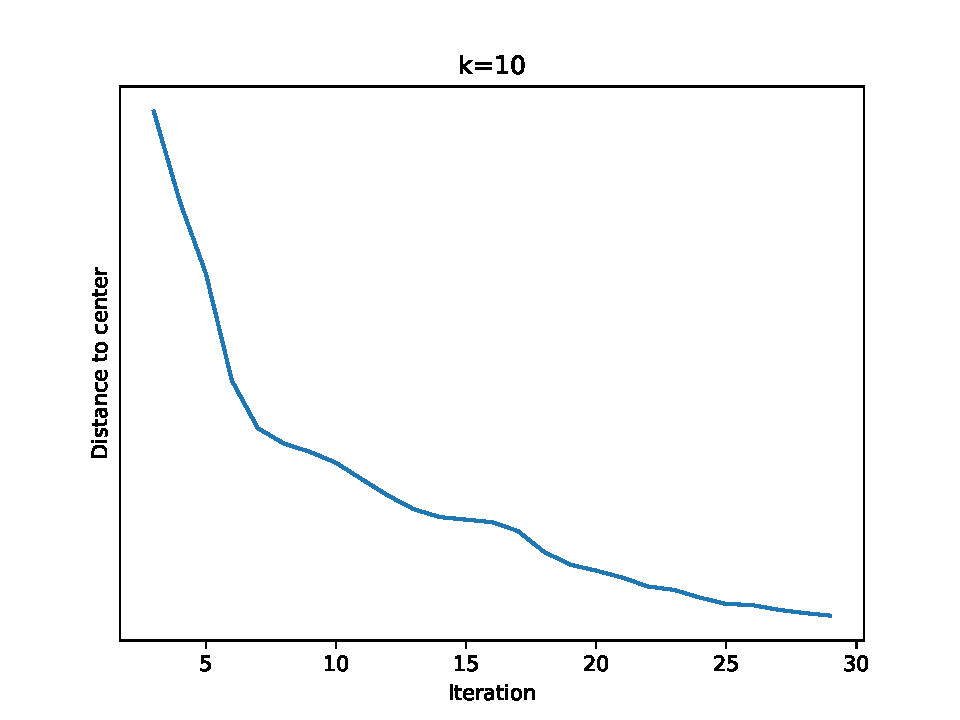
\includegraphics[width=4 in]{Figures/error++10.pdf}\\
    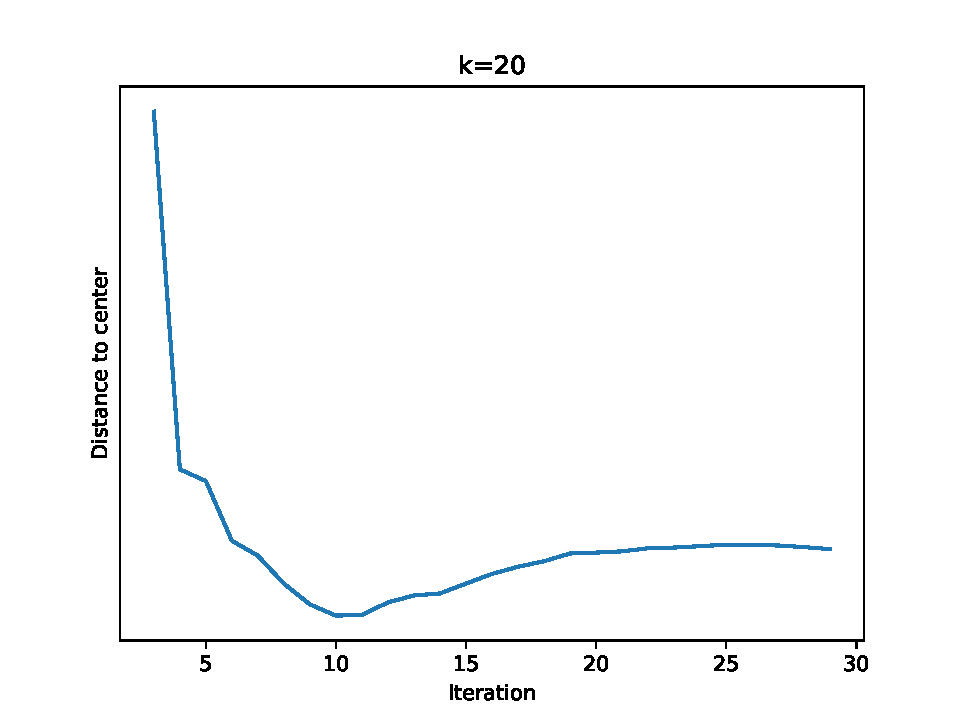
\includegraphics[width=4 in]{Figures/error++20.pdf}\\
    
    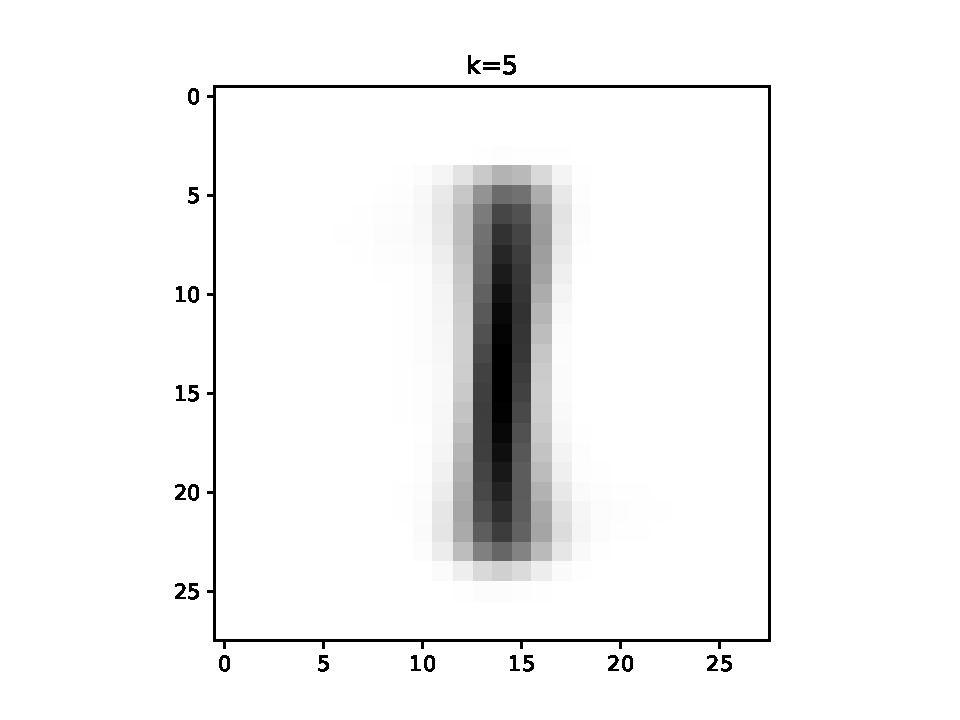
\includegraphics[width=2 in]{Figures/means++5_0.pdf}    
    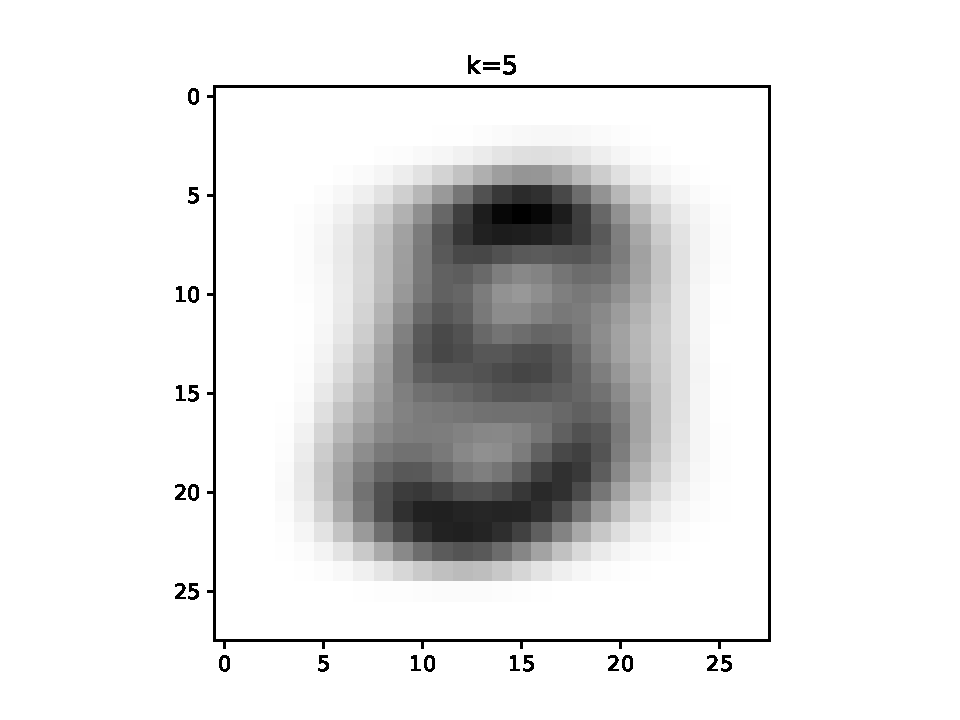
\includegraphics[width=2 in]{Figures/means++5_1.pdf}    
    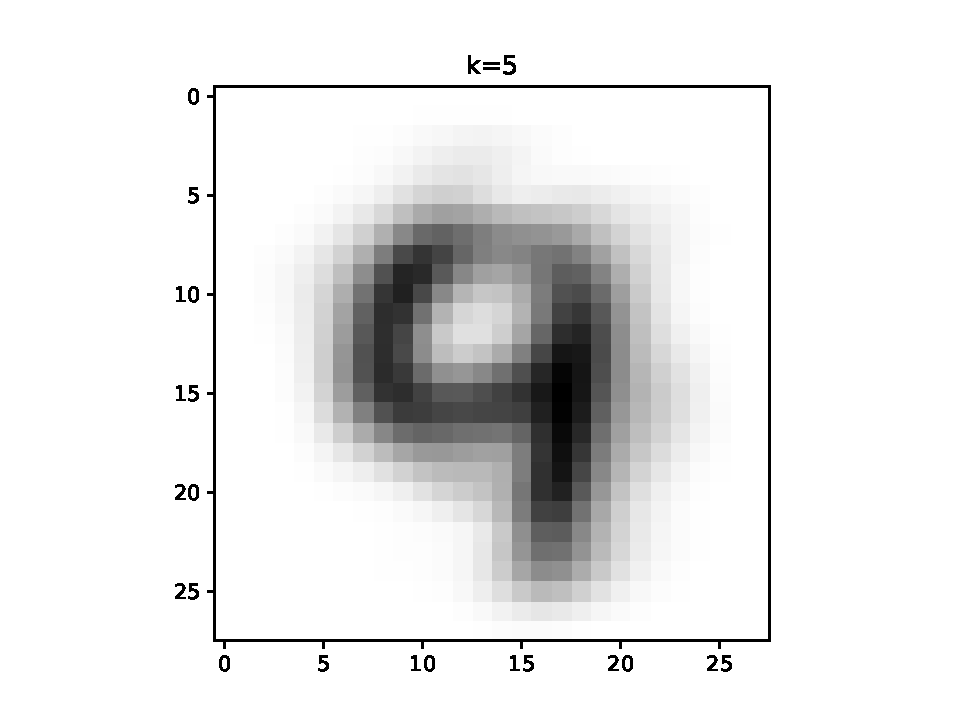
\includegraphics[width=2 in]{Figures/means++5_2.pdf}\\
     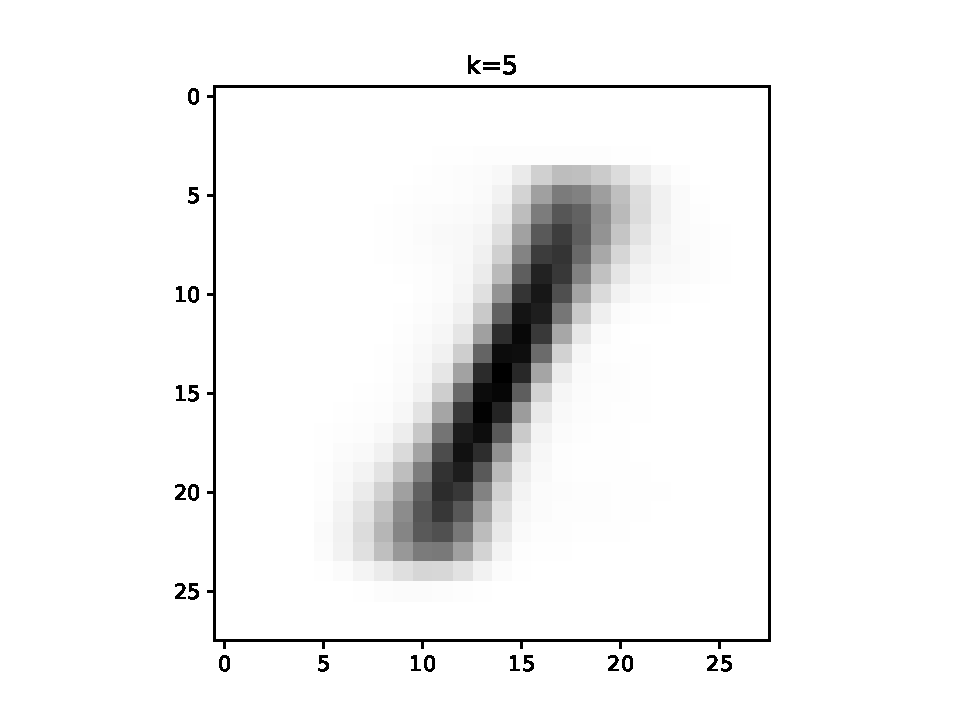
\includegraphics[width=2 in]{Figures/means++5_3.pdf}    
    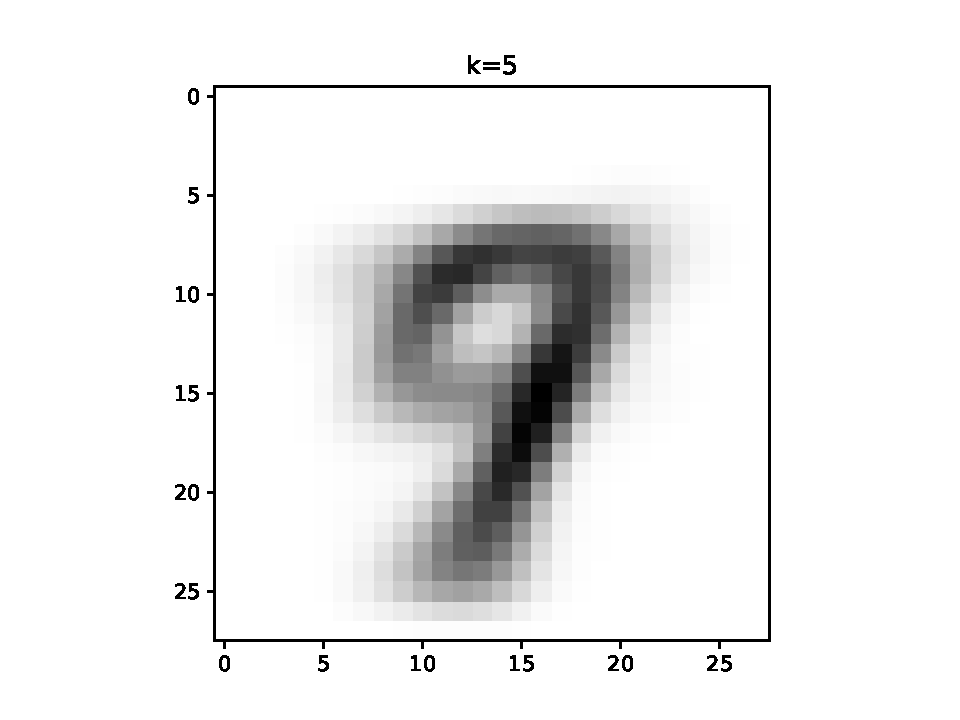
\includegraphics[width=2 in]{Figures/means++5_4.pdf} \\
    
     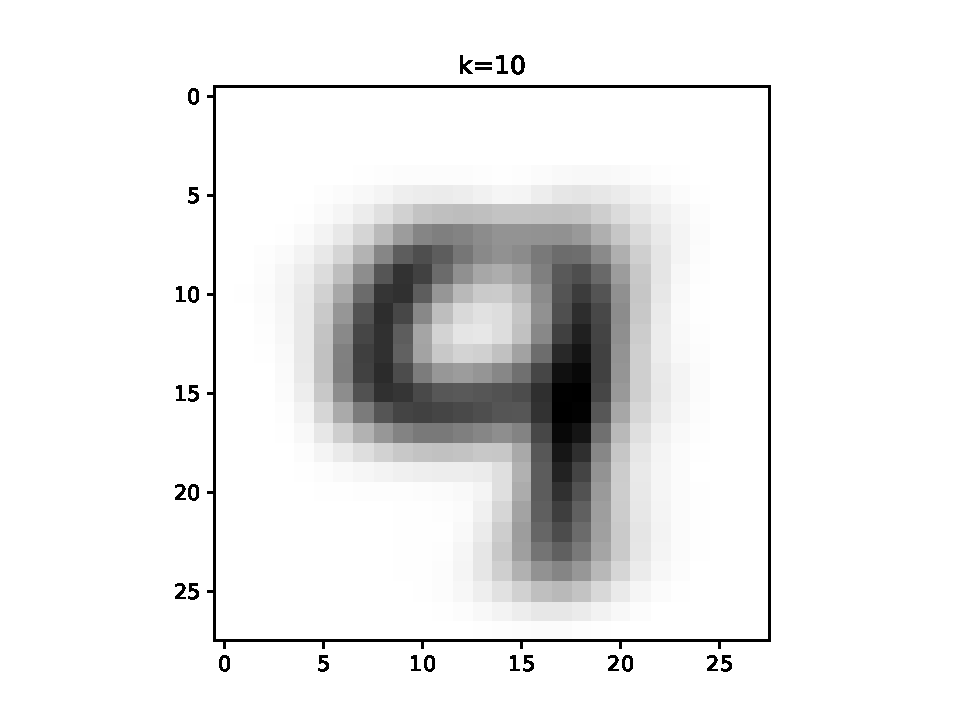
\includegraphics[width=2 in]{Figures/means++10_0.pdf}    
    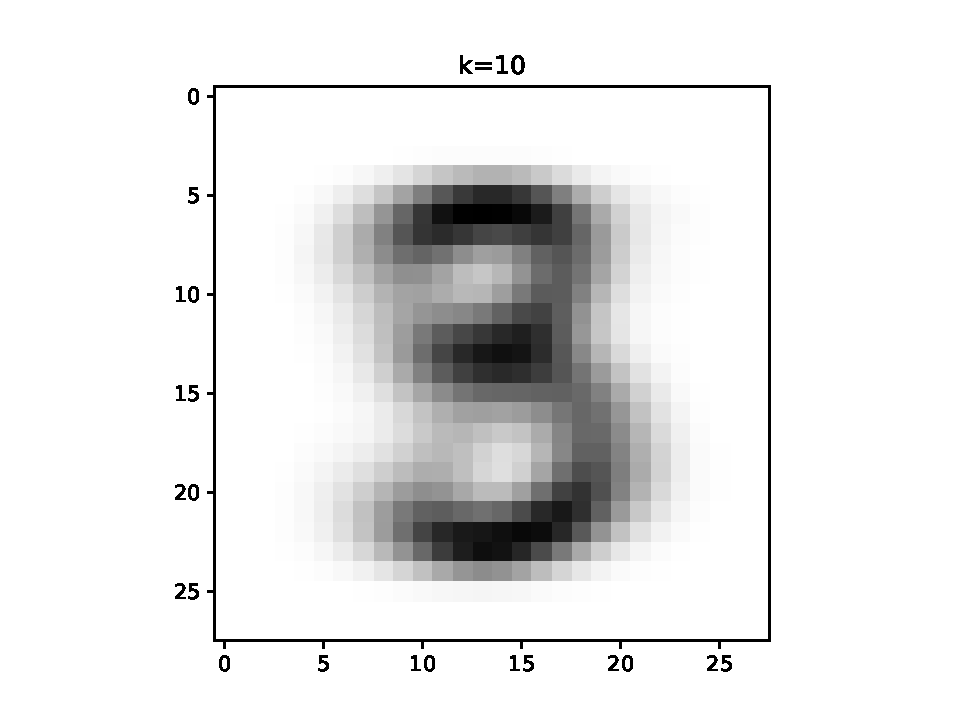
\includegraphics[width=2 in]{Figures/means++10_1.pdf}    
    \includegraphics[width=2 in]{Figures/means++10_2.pdf}\\
     \includegraphics[width=2 in]{Figures/means++10_3.pdf}    
    \includegraphics[width=2 in]{Figures/means++10_4.pdf} 
     \includegraphics[width=2 in]{Figures/means++10_5.pdf}   \\
    \includegraphics[width=2 in]{Figures/means++10_6.pdf}    
    \includegraphics[width=2 in]{Figures/means++10_7.pdf}
     \includegraphics[width=2 in]{Figures/means++10_8.pdf}    \\
    \includegraphics[width=2 in]{Figures/means++10_9.pdf} \\
    
     \includegraphics[width=2 in]{Figures/means++20_0.pdf}    
    \includegraphics[width=2 in]{Figures/means++20_1.pdf}    
    \includegraphics[width=2 in]{Figures/means++20_2.pdf}\\
     \includegraphics[width=2 in]{Figures/means++20_3.pdf}    
    \includegraphics[width=2 in]{Figures/means++20_4.pdf} 
     \includegraphics[width=2 in]{Figures/means++20_5.pdf}   \\
    \includegraphics[width=2 in]{Figures/means++20_6.pdf}    
    \includegraphics[width=2 in]{Figures/means++20_7.pdf}
     \includegraphics[width=2 in]{Figures/means++20_8.pdf}    \\
    \includegraphics[width=2 in]{Figures/means++20_9.pdf} 
       \includegraphics[width=2 in]{Figures/means++20_10.pdf}    
    \includegraphics[width=2 in]{Figures/means++20_11.pdf}    \\
    \includegraphics[width=2 in]{Figures/means++20_12.pdf}
     \includegraphics[width=2 in]{Figures/means++20_13.pdf}    
    \includegraphics[width=2 in]{Figures/means++20_14.pdf} \\
     \includegraphics[width=2 in]{Figures/means++20_15.pdf}   
    \includegraphics[width=2 in]{Figures/means++20_16.pdf}    
    \includegraphics[width=2 in]{Figures/means++20_17.pdf}\\
     \includegraphics[width=2 in]{Figures/means++20_18.pdf}  
    \includegraphics[width=2 in]{Figures/means++20_19.pdf} \\
\end{enumerate}
\textbf{Code:}
\begin{lstlisting}[language=Python]
import numpy as np
import matplotlib.pyplot as plt
from mnist import MNIST
import random

X_train = []
X_test = []
labels_test = []
labels_train = []


def load_dataset():
    global X_train, X_test, labels_test, labels_train
    mndata = MNIST('./python-mnist/data/')
    X_train, labels_train = map(np.array, mndata.load_training())
    X_test, labels_test = map(np.array, mndata.load_testing())
    X_train = X_train/255.0
    X_test = X_test/255.0


def lloyds(x, k):

    index = random.sample(range(x.shape[1]), k)
    cent = x[index]
    label = np.zeros(x.shape[0])

    # plt.figure()
    # plt.imshow(cent[1].reshape(28, 28))
    # plt.pause(0.05)
    errList = np.zeros(1)
    for l in range(30):
        err = 0
        for i in range(x.shape[0]):
            dist = np.sum((cent-x[i, :])**2, axis=1)
            label[i] = np.argmin(dist)

            err += min(dist)

        errList = np.append(errList, err)

        for j in range(k):
            if (x[label == j].size) > 0:
                cent[j] = np.sum(x[label == j], axis=0)/(x[label == j].size)

        # plt.imshow(cent[0].reshape(28, 28))
        # plt.pause(0.05)

    plt.figure()
    plt.plot(range(3,30), errList[4:])
    plt.xlabel('Iteration')
    plt.ylabel('Distance to center')
    plt.yscale('log')
    plt.title('k='+str(k))
    plt.savefig('Figures/error' + str(k) + '.pdf')

    for p in range(k):

        plt.figure()
        plt.imshow(cent[p].reshape(28, 28))
        plt.title('k=' + str(k))
        plt.set_cmap('gray_r')
        plt.savefig('Figures/means'+str(k)+'_'+str(p)+'.pdf')


def kmeanspp(x, k):

    index = random.sample(range(x.shape[1]), 1)
    cent = x[index]

    for o in range(1,k):
        prob = np.zeros(x.shape[0])

        for i in range(x.shape[0]):
            dist = np.sum((cent - x[i, :]) ** 2, axis=1)
            prob[i] = np.min(dist) ** 2 / np.sum(dist ** 2)

        prob /= np.sum(prob)

        cent = np.concatenate((cent, x[np.random.choice(range(x.shape[0]), 1, p=prob)]))

    label = np.zeros(x.shape[0])

    # plt.figure()
    # plt.imshow(cent[1].reshape(28, 28))
    # plt.pause(0.05)
    errList = np.zeros(1)
    for l in range(30):
        err = 0
        for i in range(x.shape[0]):
            dist = np.sum((cent-x[i, :])**2, axis=1)
            label[i] = np.argmin(dist)
            prob[i] = np.min(dist)**2/np.sum(dist**2)
            err += min(dist)

        errList = np.append(errList, err)

        for j in range(k):
            if (x[label == j].size) > 0:
                cent[j] = np.sum(x[label == j], axis=0)/(x[label == j].size)

        # plt.imshow(cent[0].reshape(28, 28))
        # plt.pause(0.05)

    plt.figure()
    plt.plot(range(3,30), errList[4:])
    plt.xlabel('Iteration')
    plt.ylabel('Distance to center')
    plt.yscale('log')
    plt.title('k='+str(k))
    plt.savefig('Figures/error++' + str(k) + '.pdf')

    for p in range(k):

        plt.figure()
        plt.imshow(cent[p].reshape(28, 28))
        plt.title('k=' + str(k))
        plt.set_cmap('gray_r')
        plt.savefig('Figures/means++'+str(k)+'_'+str(p)+'.pdf')


load_dataset()

kList=[5, 10, 20]
for k in kList:
    lloyds(X_train, k)
    kmeanspp(X_train, k)
\end{lstlisting}


\section{Joke Recommender System}

5. \grade{8} You will build a personalized joke recommender system. There are $m = 100$ jokes and $n = 24,983$ users\footnote{Data from \url{http://eigentaste.berkeley.edu/dataset/}}. As historical data, every user read a subset of jokes and rated them. The goal is to recommend more jokes, such that the recommended jokes match the individual user's sense of humor.
The historical rating is represented by a matrix $R\in \R^{n \times m}$. The entry $R_{i,j}$ represents the user $i$'s rating on joke $j$. The rating is a real number in $[-10,10]$: a higher value represents that the user is more satisfied with the joke.
The directory $\tt /jokes$ contains the text of all $100$ jokes. Read them before you start! In addition, you are provided with two files:
\begin{itemize}
\item $\tt train.txt$ contains the joke-user-score data representing the training set. Each line takes the form ``$\tt i,j,s$'', where $\tt i$ is the user index, $\tt j$ is the joke index, and $\tt s$ is the user's score in $[-10,10]$ describing how much they liked the joke (higher is better).
\item $\tt test.txt$ has the same format, with the same users rating movies held out from the training set.
\end{itemize}

Latent factor model is the state-of-the-art method for personalized recommendation. It learns a vector representation $u_i\in \R^d$ for each user and a vector representation $v_j\in \R^d$ for each joke, such that
the inner product $\langle u_i,v_j\rangle$ approximates the rating~$R_{i,j}$. You will build a simple latent factor model.
We will evaluate our learnt vector representations by two metrics
\begin{itemize}
  \item Mean squared error: $\frac{1}{|S|} \sum_{(i,j)\in S} (\langle u_i,v_j\rangle - R_{ij})^2$ where $S$ (and the corresponding $R_{i,j}$ values) are from the test set
  \item Mean absolute error: $\frac{1}{n} \sum_{i=1}^n \frac{1}{|\mathcal{N}_i|} \sum_{j \in \mathcal{N}_i} |\langle u_i,v_j\rangle - R_{ij}|$ where $\mathcal{N}_i$ are the jokes rated by user $i$ in the test set
\end{itemize}  

You will implement multiple estimators and use the inner product $\langle u_i,v_j\rangle$ to predict if user $i$ likes joke $j$ in the test data.
You will choose hyperparameters like $d$ or the amount of regularization by creating a validation set from the training set.

\begin{enumerate}
\item The first estimator pools all the users together and just predicts what the average user in the training set rated the joke. This is equivalent to $d=1$ with $u$ as the all ones vector and $v$ minimizing least squares.    

\textbf{Answer:}\\
Average User Error: 279.3989927124748

\item Now replace all missing values in $R_{i,j}$ no in the training set by zero. Then use singular value decomposition (SVD) to learn a lower dimensional vector representation for users and jokes. Recall this means to project the data vectors to lower dimensional subspaces of their corresponding spaces, spanned by singular vectors. Refer to the lecture materials on SVD, PCA and dimensionality reduction. You should use an efficient solver, I recommend \texttt{scipy.sparse.linalg.svds}. Try $d=1,2,5,10,20,50$ and plot the error metrics on the train and test as a function of $d$. 

\textbf{Answer:}\\
\includegraphics[width=4 in]{Figures/svd_err_mse.pdf}

\item For sparse data, replacing all missing values by zero is not a completely satisfying solution. A missing value means that the user has not read the joke, but doesn't mean that the rating should be zero. A more reasonable choice is to minimize the MSE only on rated jokes. Let's define a loss function:
\[
  L\Big(\{u_i\},\{v_j\}\Big) := \sum_{(i,j)\in T} (\langle u_i,v_j\rangle - R_{i,j})^2
  + \lambda \sum_{i=1}^n \|u_i\|_2^2 + \lambda \sum_{j=1}^m \|v_j\|_2^2,
\]
where $T$ and $R_{i,j}$ here are from the training set and $\lambda > 0$ is the regularization coefficient. Implement an algorithm to learn vector representations by minimizing the loss function $L(\{u_i\},\{v_j\})$.
Try $d=1,2,5,10,20,50$ and plot the error metrics on the train and test as a function of $d$. 
Note that you may need to tune the hyper-parameter $\lambda$ to optimize the performance.

{\bf Hint:} you may want to employ an alternating minimization scheme. First, randomly initialize $\{u_i\}$ and $\{v_j\}$. Then minimize the loss function with respective to $\{u_i\}$ by treating $\{v_j\}$ as constant vectors, and minimize the loss function with respect to $\{v_j\}$ by treating $\{u_i\}$ as constant vectors. Iterate these two steps until both $\{u_i\}$ and $\{v_j\}$ converge. Note that when one of $\{u_i\}$ or $\{v_j\}$ is given, minimizing the loss function with respect to the other part has closed-form solutions. You should never be allocating an $m \times n$ matrix for this problem. 

\textbf{Answer:}\\
\includegraphics[width=4 in]{Figures/loss_err_mse.pdf}  

\textbf{Code:}
\begin{lstlisting}[language=Python]
import numpy as np
import matplotlib.pyplot as plt
from scipy.sparse import dok_matrix
from scipy.sparse.linalg import svds


def read_data():

    test = dok_matrix((24983, 100), dtype=np.float32)
    train = dok_matrix((24983, 100), dtype=np.float32)
    val = dok_matrix((24983, 100), dtype=np.float32)

    f = open('test.txt', 'r')
    for line in f.readlines():
        nums = line.split(',')
        test[int(nums[0])-1, int(nums[1])-1] = float(nums[2])

    f.close()

    f = open('train.txt', 'r')
    for line in f.readlines():
        nums = line.split(',')
        ran = np.random.uniform(0, 10, 1)
        if ran <= 8:
            train[int(nums[0])-1, int(nums[1])-1] = float(nums[2])
        if ran > 8:
            val[int(nums[0]) - 1, int(nums[1]) - 1] = float(nums[2])
    f.close()

    return test, train, val


def av_user_estimator(R):

    ons = np.ones((1, R.shape[0]))

    v = ons*R/ons.size
    return v


def svd_series(test, train):

    R_test=test.todense()
    R_train = train.todense()

    dList = [1, 2, 5, 10, 20, 50]

    train_err_mse = np.zeros(1)
    test_err_mse = np.zeros(1)
    train_err_mae = np.zeros(1)
    test_err_mae = np.zeros(1)

    N_train = np.sum(R_train != 0, axis=1)
    N_test = np.sum(R_test != 0, axis=1)

    for d in dList:
        u, s, vt = svds(R_train, k=d)

        train_err_mse = np.append(train_err_mse, np.sum(np.sum(np.square(np.dot(u, vt) - R_train)))/train.nnz)
        test_err_mse = np.append(test_err_mse, np.sum(np.sum(np.square(np.dot(u, vt) - R_test)))/test.nnz)

        train_err_mae = np.append(train_err_mae, np.sum(np.sum(np.divide(np.absolute(np.dot(u, vt) - R_train), N_train))) / R_train.shape[0])
        test_err_mae = np.append(test_err_mae, np.sum(np.sum(np.divide(np.absolute(np.dot(u, vt) - R_test), N_test))) / R_test.shape[0])

    plt.figure()
    plt.plot(dList, train_err_mse[1:])
    plt.plot(dList, test_err_mse[1:])
    plt.xlabel('d')
    plt.ylabel('Error')
    plt.legend(('Training Error', 'Testing Error'))
    plt.title('Mean Squared Error')
    plt.savefig('Figures/svd_err_mse.pdf')
    plt.draw()

    plt.figure()
    plt.plot(dList, train_err_mae[1:])
    plt.plot(dList, test_err_mae[1:])
    plt.xlabel('d')
    plt.ylabel('Error')
    plt.legend(('Training Error', 'Testing Error'))
    plt.title('Mean Absolute Error')
    plt.savefig('Figures/svd_err_mae.pdf')
    plt.draw()


def loss_min(train, d, lamb):

    u = np.random.randn(train.shape[0], d)

    lastErr = 10**100
    for i in range(20):
        if i % 2 == 0:
            v = np.linalg.solve(np.dot(u.T, u) + lamb, u.T*train)

        else:
            u = np.linalg.solve(np.dot(v, v.T) + lamb, (train*v.T).T).T

        if np.sum(np.sum(np.dot((np.dot(u, v) - train).T, (np.dot(u, v) - train)))) > lastErr:
            break

        lastErr = np.sum(np.sum(np.dot((np.dot(u, v) - train).T, (np.dot(u, v) - train))))

        print(i, lastErr)

    return u, v

def loss_reg(test, train, val, d):

    lamb_Vec = range(10)
    err = np.zeros(1)
    for lamb in lamb_Vec:
        u, v = loss_min(train, d, lamb)
        err = np.append(err, np.sum(np.dot((np.dot(u, v) - train).T, (np.dot(u, v) - train))))

    plt.plot(lamb_Vec, err[1:])
    plt.draw()


test, train, val = read_data()

v = av_user_estimator(train)
ons = np.ones((1, test.shape[0]))
err = np.sum(ons.size * v.T * v - v.T * ons * test - test.T * ons.T * v + test.T * test) / test.nnz
print('Average User Error: '+str(err))

svd_series(test, train)

loss_reg(test, train, val, 3)

dList=[1, 2, 5, 10, 20, 50]
errTest=np.zeros(1)
errTrain=np.zeros(1)
for d in dList:
    u, v = loss_min(train, d, 10)
    errTrain = np.append(errTrain, np.sum(np.sum(np.square(np.dot(u, v) - train)))/train.nnz)
    errTest = np.append(errTest, np.sum(np.sum(np.square(np.dot(u, v) - test)))/test.nnz)

plt.figure()
plt.plot(dList, errTrain[1:])
plt.plot(dList, errTest[1:])
plt.xlabel('d')
plt.ylabel('Error')
plt.legend(('Training Error', 'Testing Error'))
plt.title('Mean Squared Error')
plt.savefig('Figures/loss_err_mse.pdf')
plt.draw()

plt.show()

\end{lstlisting}

\end{enumerate}



\end{document}
